%% ---------------------------------------------------------------------------
%% 4. Numerical results
%% ---------------------------------------------------------------------------
\section{Numerical results}\label{sec:numerical}

\subsection{Examination for integration consistency}\label{sec:consistency}

As stated in Section \ref{sec:error}, the integration consistency of an integration method plays a crucial role in the convergence performance.
Consequently, for subsequent development, we investigate and examine the integration consistency by manufactured problems with polynomial solutions:
\begin{equation}\label{eq:89}
w=\left(\sum_{i=1}^{n_{sd}}x_i+1\right)^{p}
\end{equation}

\begin{figure}[pos=htbp]
\centering
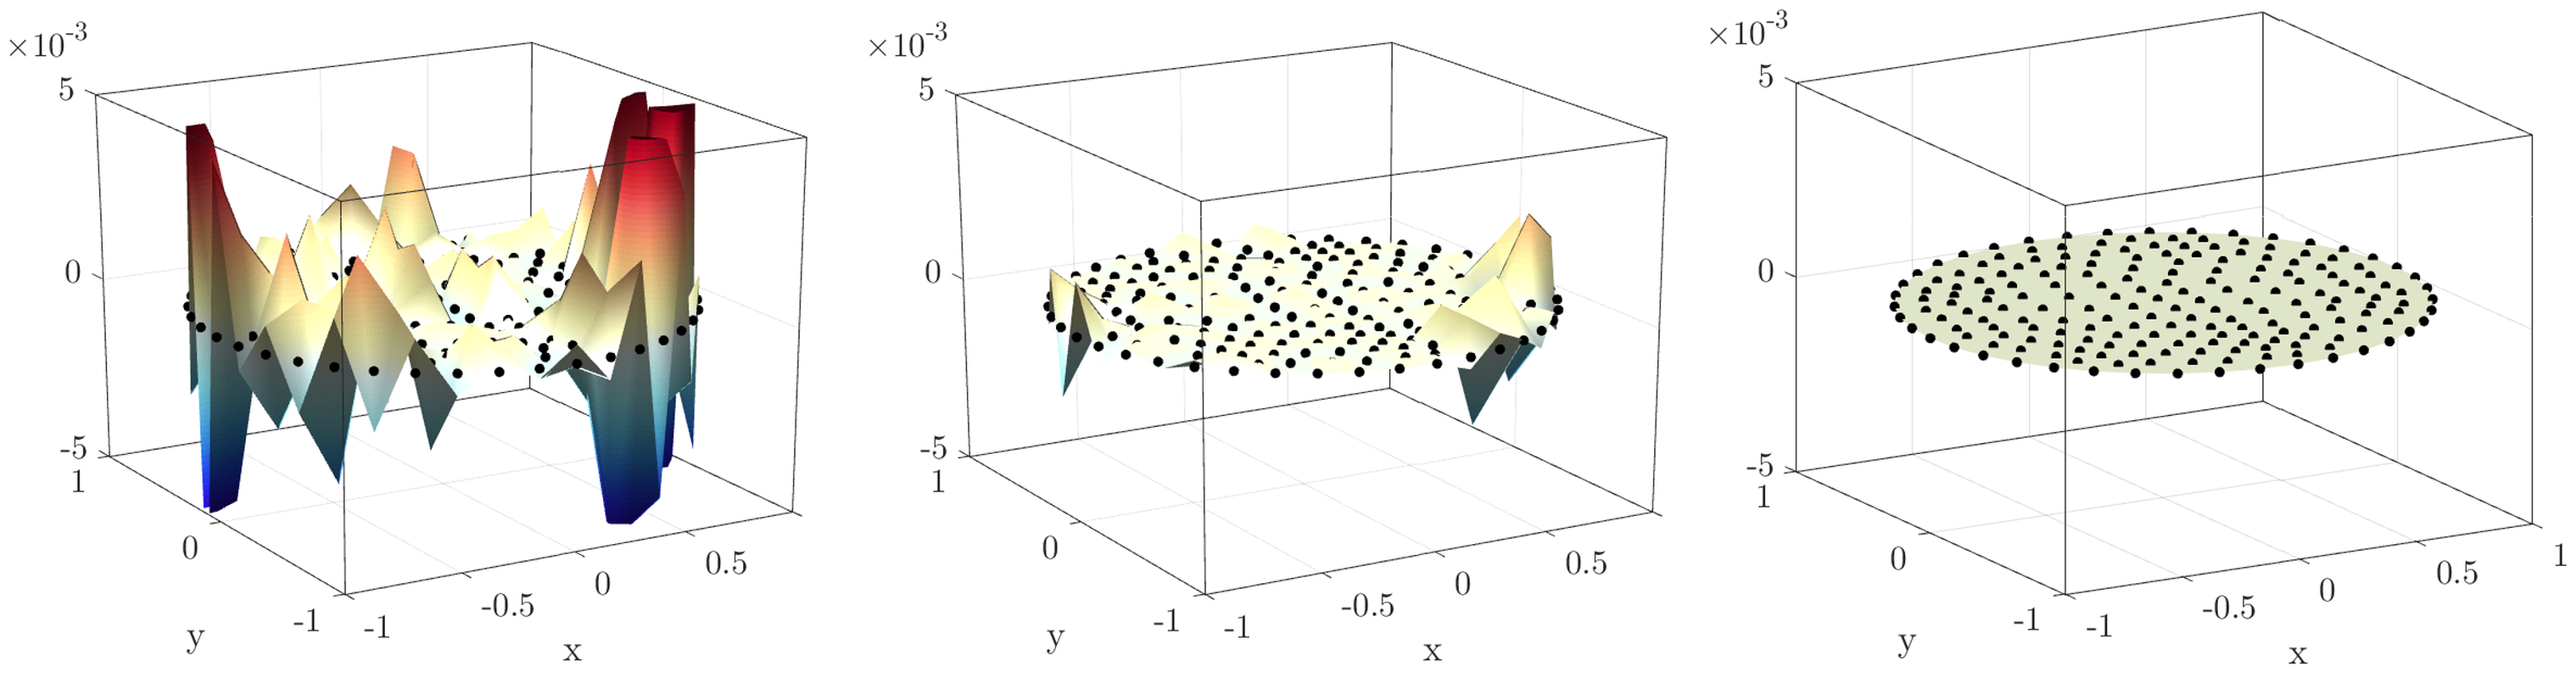
\includegraphics[width=\textwidth]{figs/fig01.png}
\caption{Examination of the 2nd order integration consistency for 2D cubic meshfree formulation.}\label{fig:1}
\end{figure}

\begin{figure}[pos=htbp]
\centering
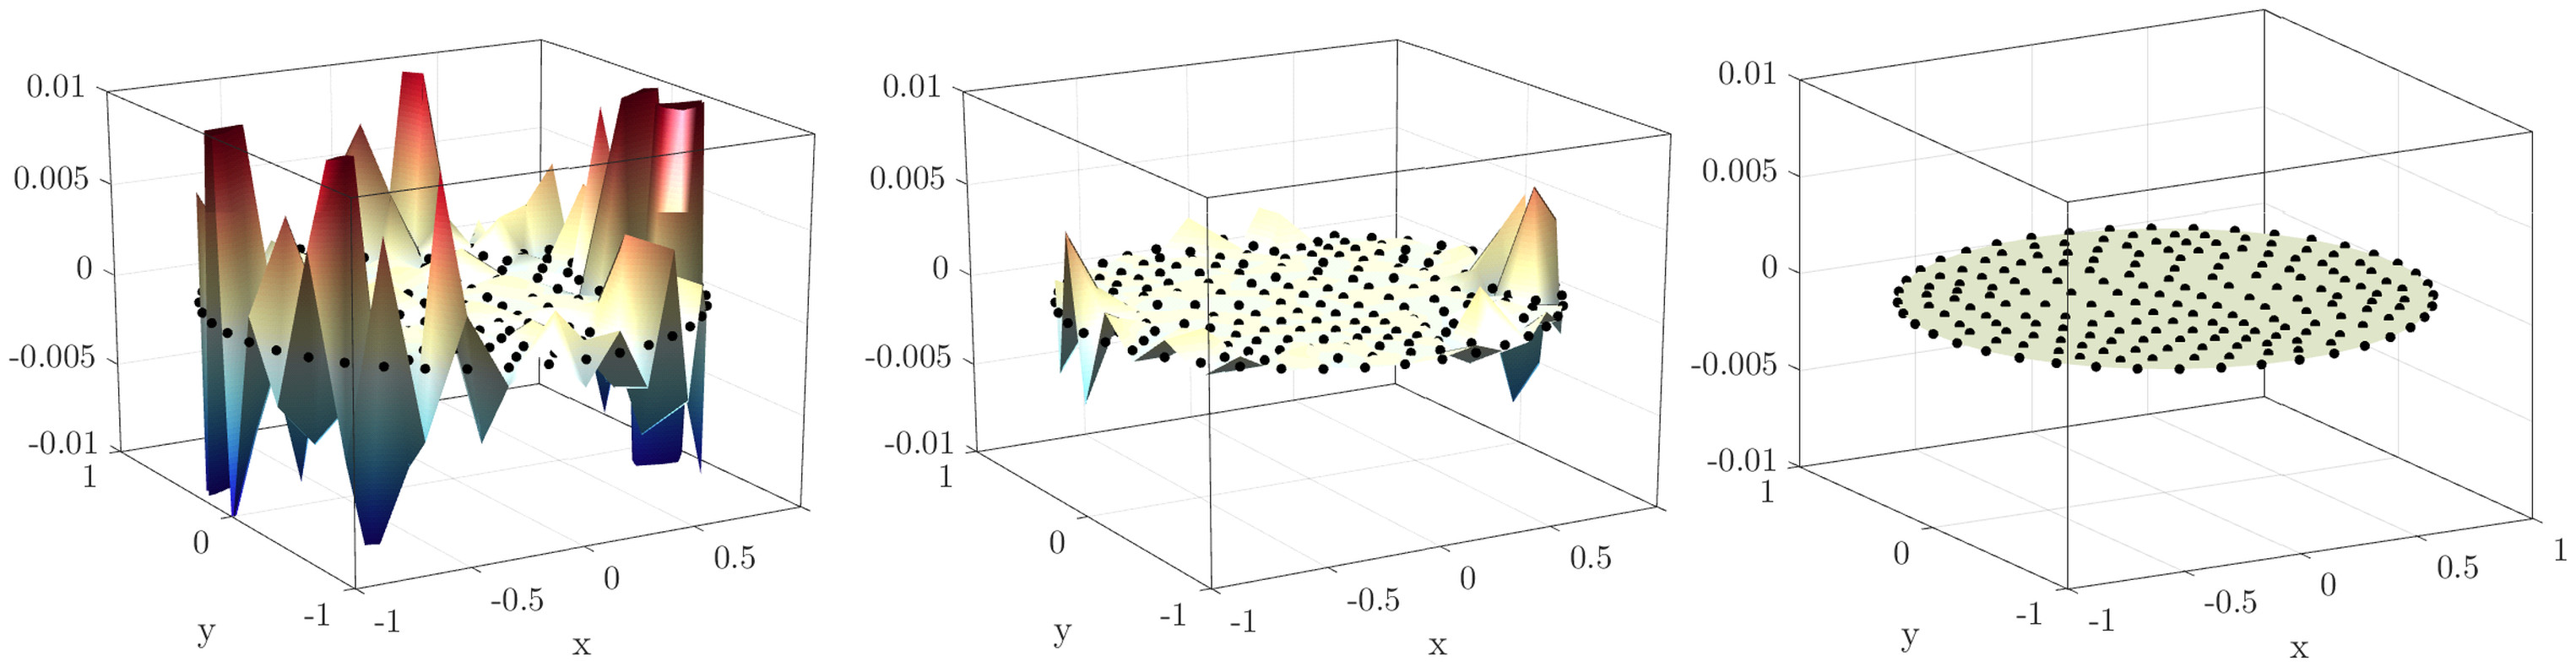
\includegraphics[width=\textwidth]{figs/fig02.png}
\caption{Examination of the 3rd order integration consistency for 2D cubic meshfree formulation.}\label{fig:2}
\end{figure}

\begin{figure}[pos=htbp]
\centering
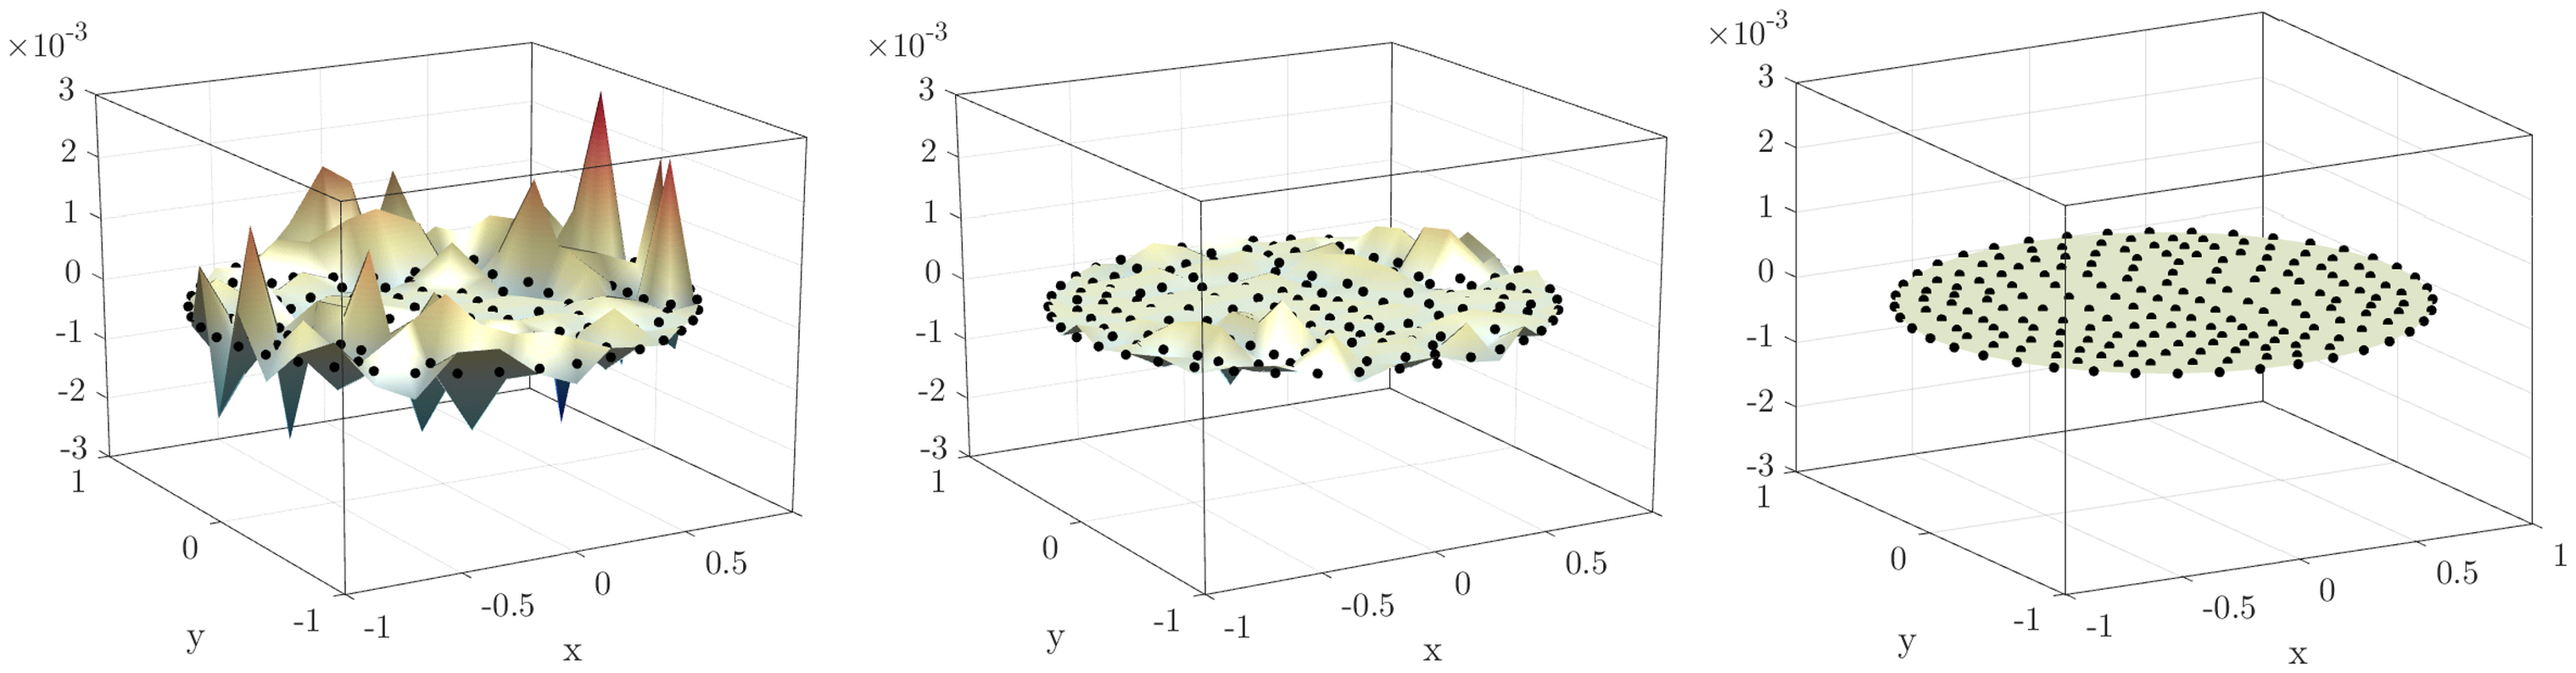
\includegraphics[width=\textwidth]{figs/fig03.png}
\caption{Examination of the 3rd order integration consistency for 2D quartic meshfree formulation.}\label{fig:3}
\end{figure}

\begin{figure}[pos=htbp]
\centering
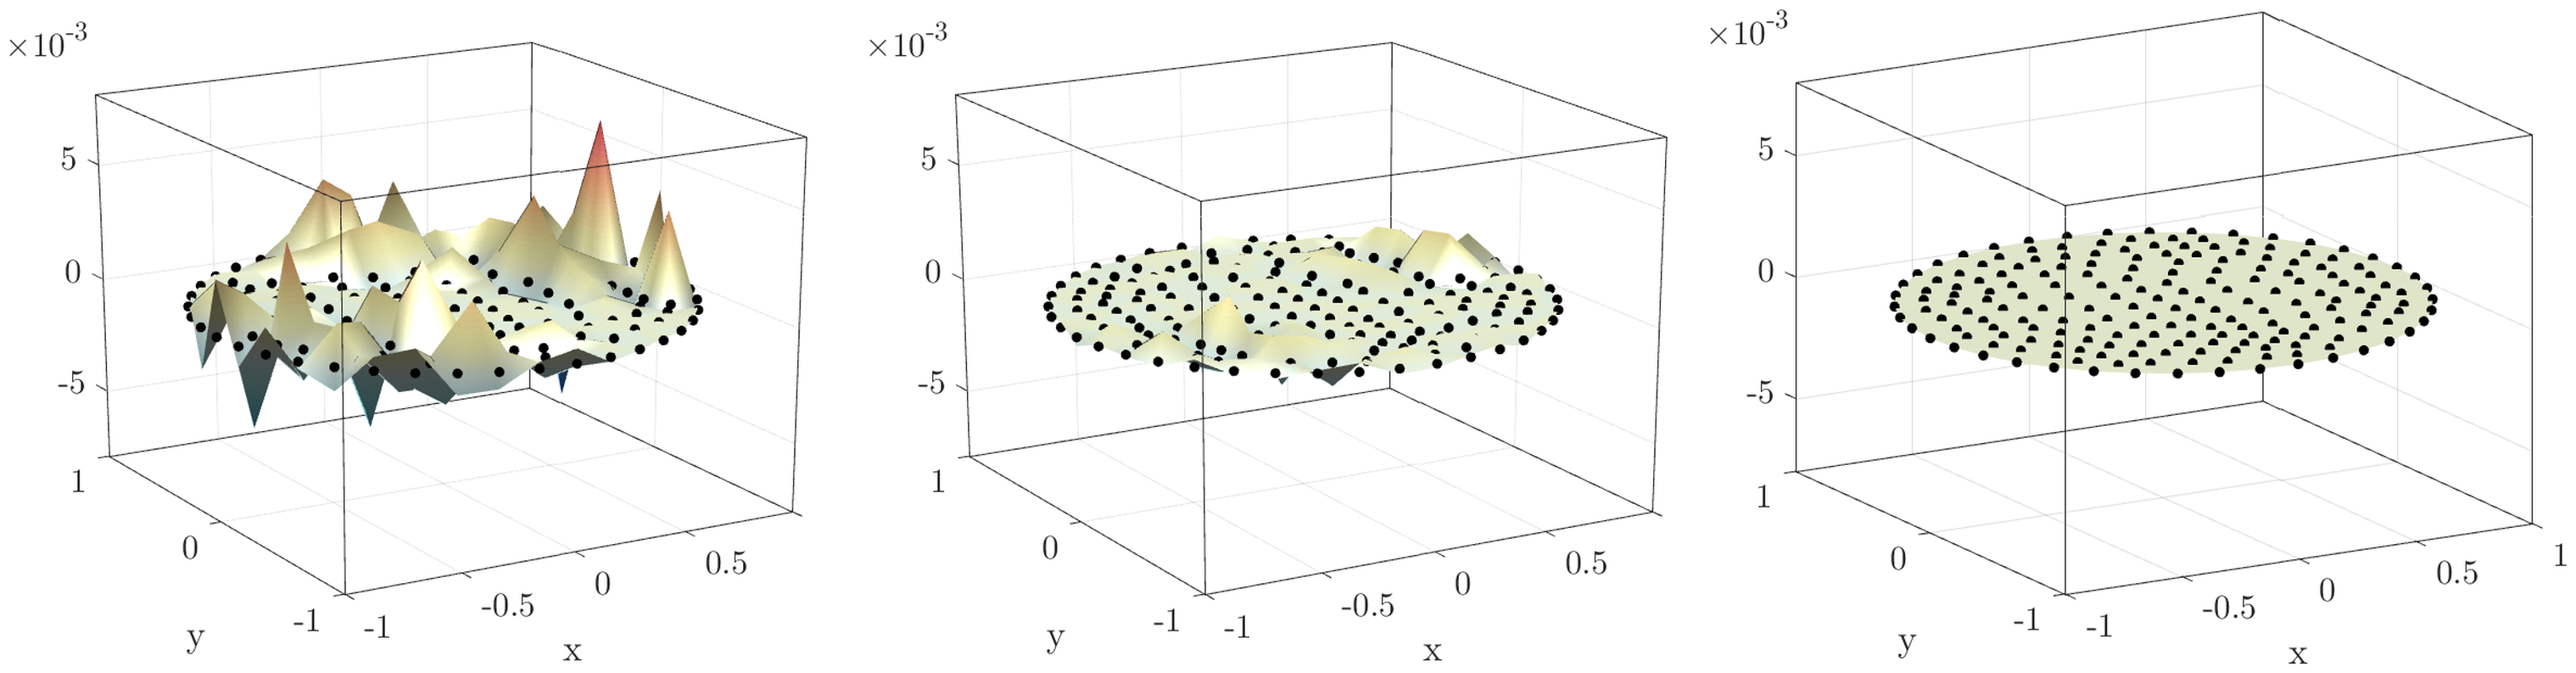
\includegraphics[width=\textwidth]{figs/fig04.png}
\caption{Examination of the 4th order integration consistency for 2D quartic meshfree formulation.}\label{fig:4}
\end{figure}

Figs. \ref{fig:1}--\ref{fig:4} clearly show the various orders of integration consistency of GI and RKGSI for cubic and quartic basis function.
Since RKGSI was generated from integration constraints of weak forms regarding to various orders $q$ of meshfree formulations, it naturally possess the integration consistency the same degree of basis functions.

\subsection{Examination for convergence rates of quadratic meshfree formulation}\label{sec:quadratic}

As stated in Section \ref{sec:error}, only when the order of basis function satisfy the minimum requirement $p\ge3$, can the $L_2$ error of various integral schemes achieves optimal convergence performance $p+1$, otherwise, only $p$th order convergence rate of $L_2$ error can be ensured when $p=2$.
Then two benchmark problems will be adopted to test the above theoretical convergence value.

We consider a 1D cantilever beam as shown in Fig. \ref{fig:5}.
The analytical solution and corresponding boundary conditions are as follows:
\begin{equation}\label{eq:90}
\begin{cases}
w=\sin x-x\\[2pt]
w(0)=0,\quad \theta(0)=0
\end{cases}
\end{equation}
The material and geometry properties of this problem are: flexural rigidity $D=2\times10^{4}$, Poisson's ratio $\nu=0.3$, length $L=10$.
The left boundary is subject to displacement and rotation boundary conditions, which are imposed by Nitsche's method.
Six regular meshfree discretizations with $11$, $21$, $41$, $81$, $161$, $321$ nodes are adopted to observe the convergence performance.
For quadratic meshfree computation, the normalized support size is set as 2.6.

\begin{figure}[pos=htbp]
\centering
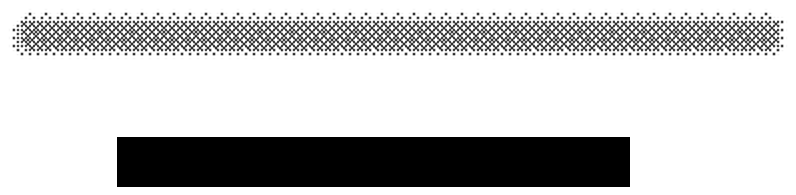
\includegraphics[width=0.7\textwidth]{figs/fig05.png}
\caption{Description of 1D cantilever beam.}\label{fig:5}
\end{figure}

\begin{figure}[pos=htbp]
\centering
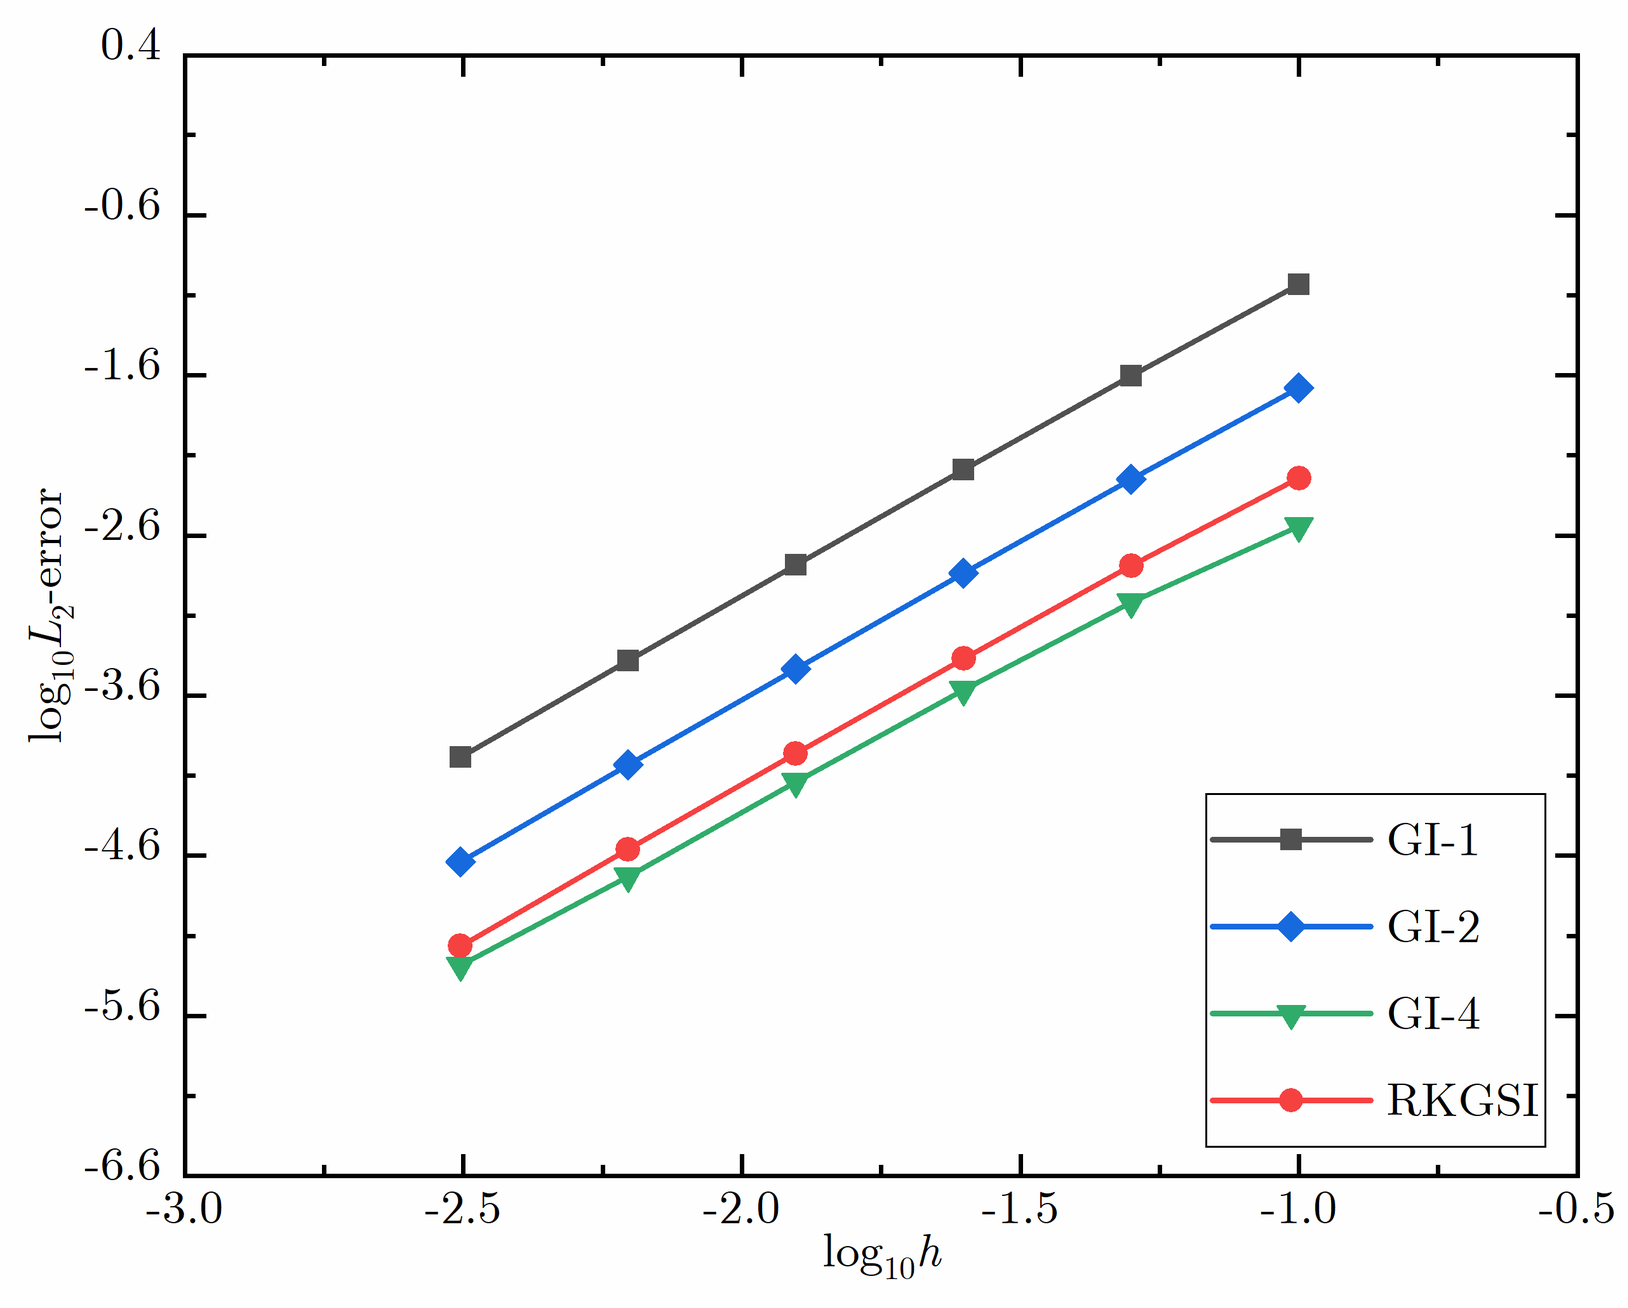
\includegraphics[width=0.55\textwidth]{figs/fig06.png}
\caption{$L_2$-error comparison for the 1D cantilever beam with $p=2$.}\label{fig:6}
\end{figure}

\begin{figure}[pos=htbp]
\centering
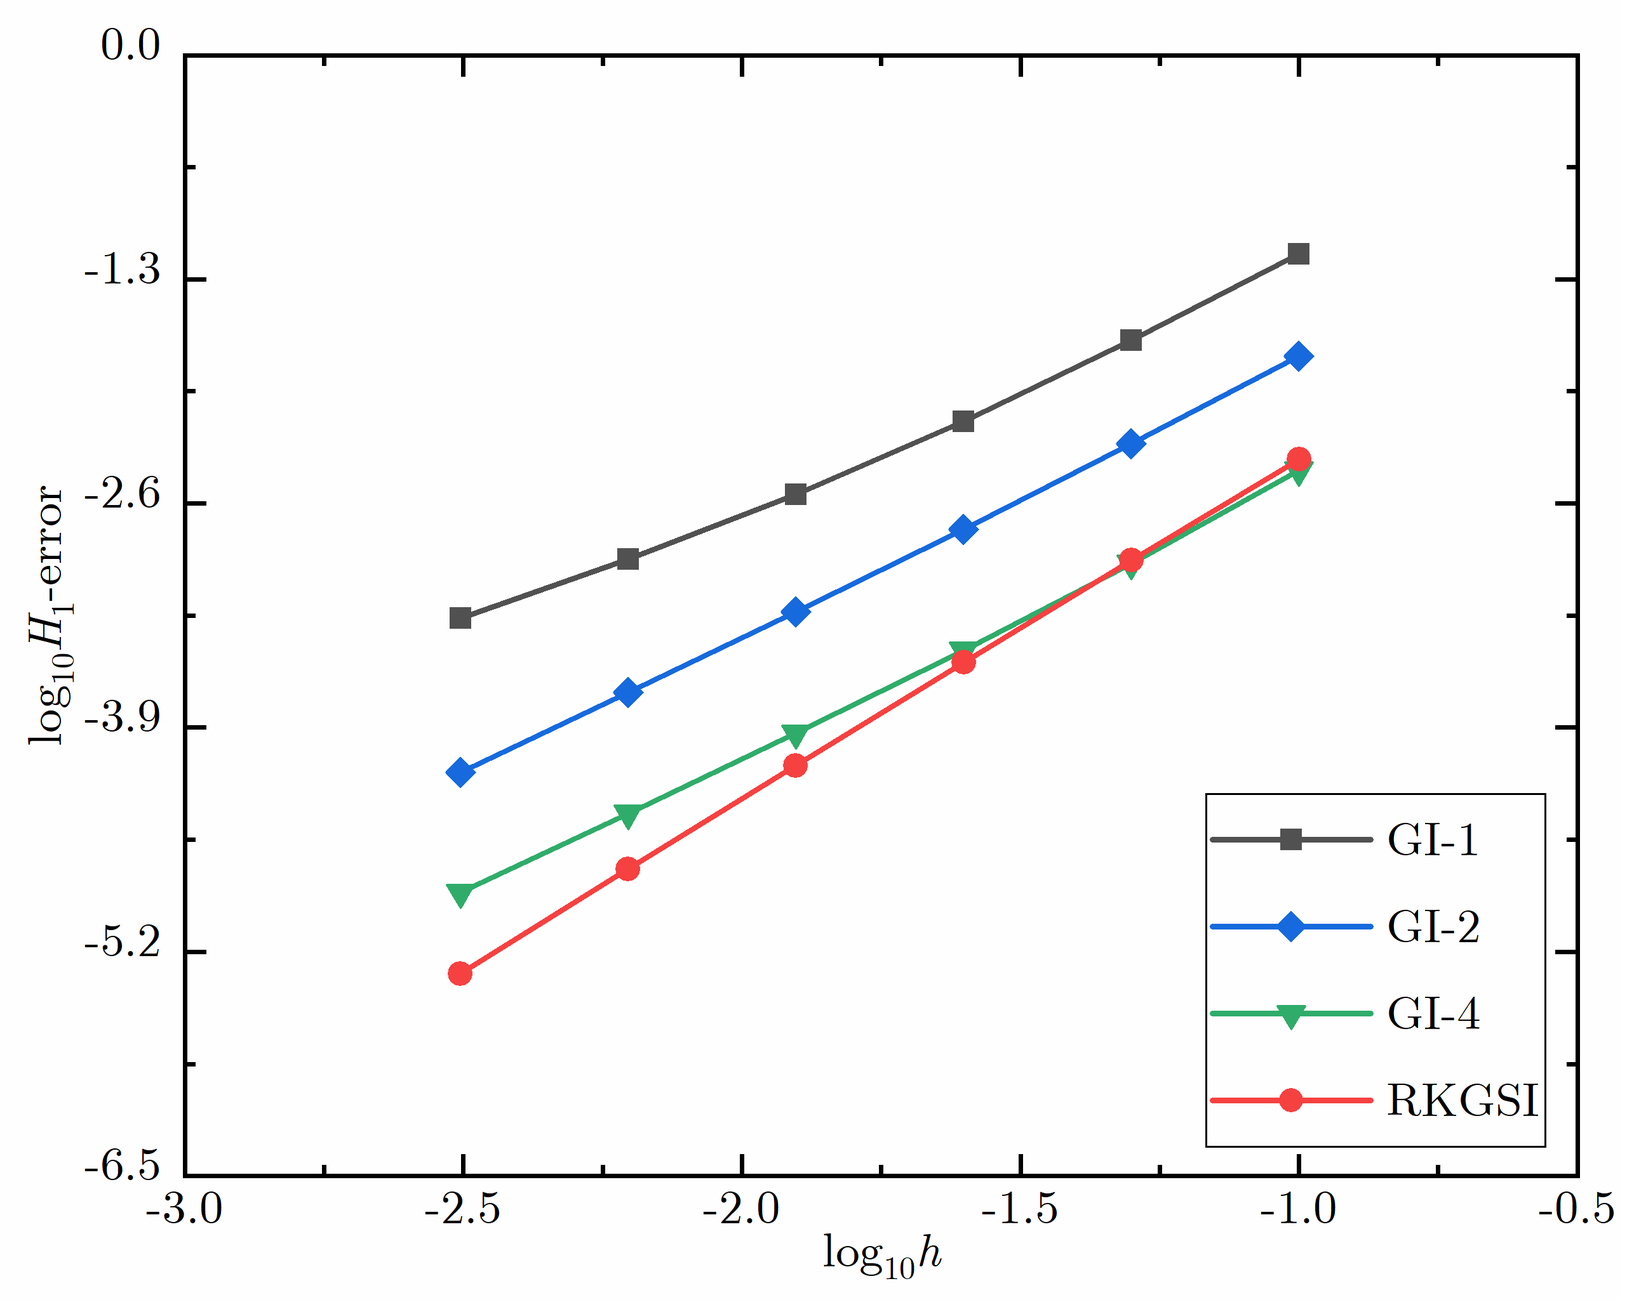
\includegraphics[width=0.55\textwidth]{figs/fig07.png}
\caption{$H_1$-error comparison for the 1D cantilever beam with $p=2$.}\label{fig:7}
\end{figure}

\begin{figure}[pos=htbp]
\centering
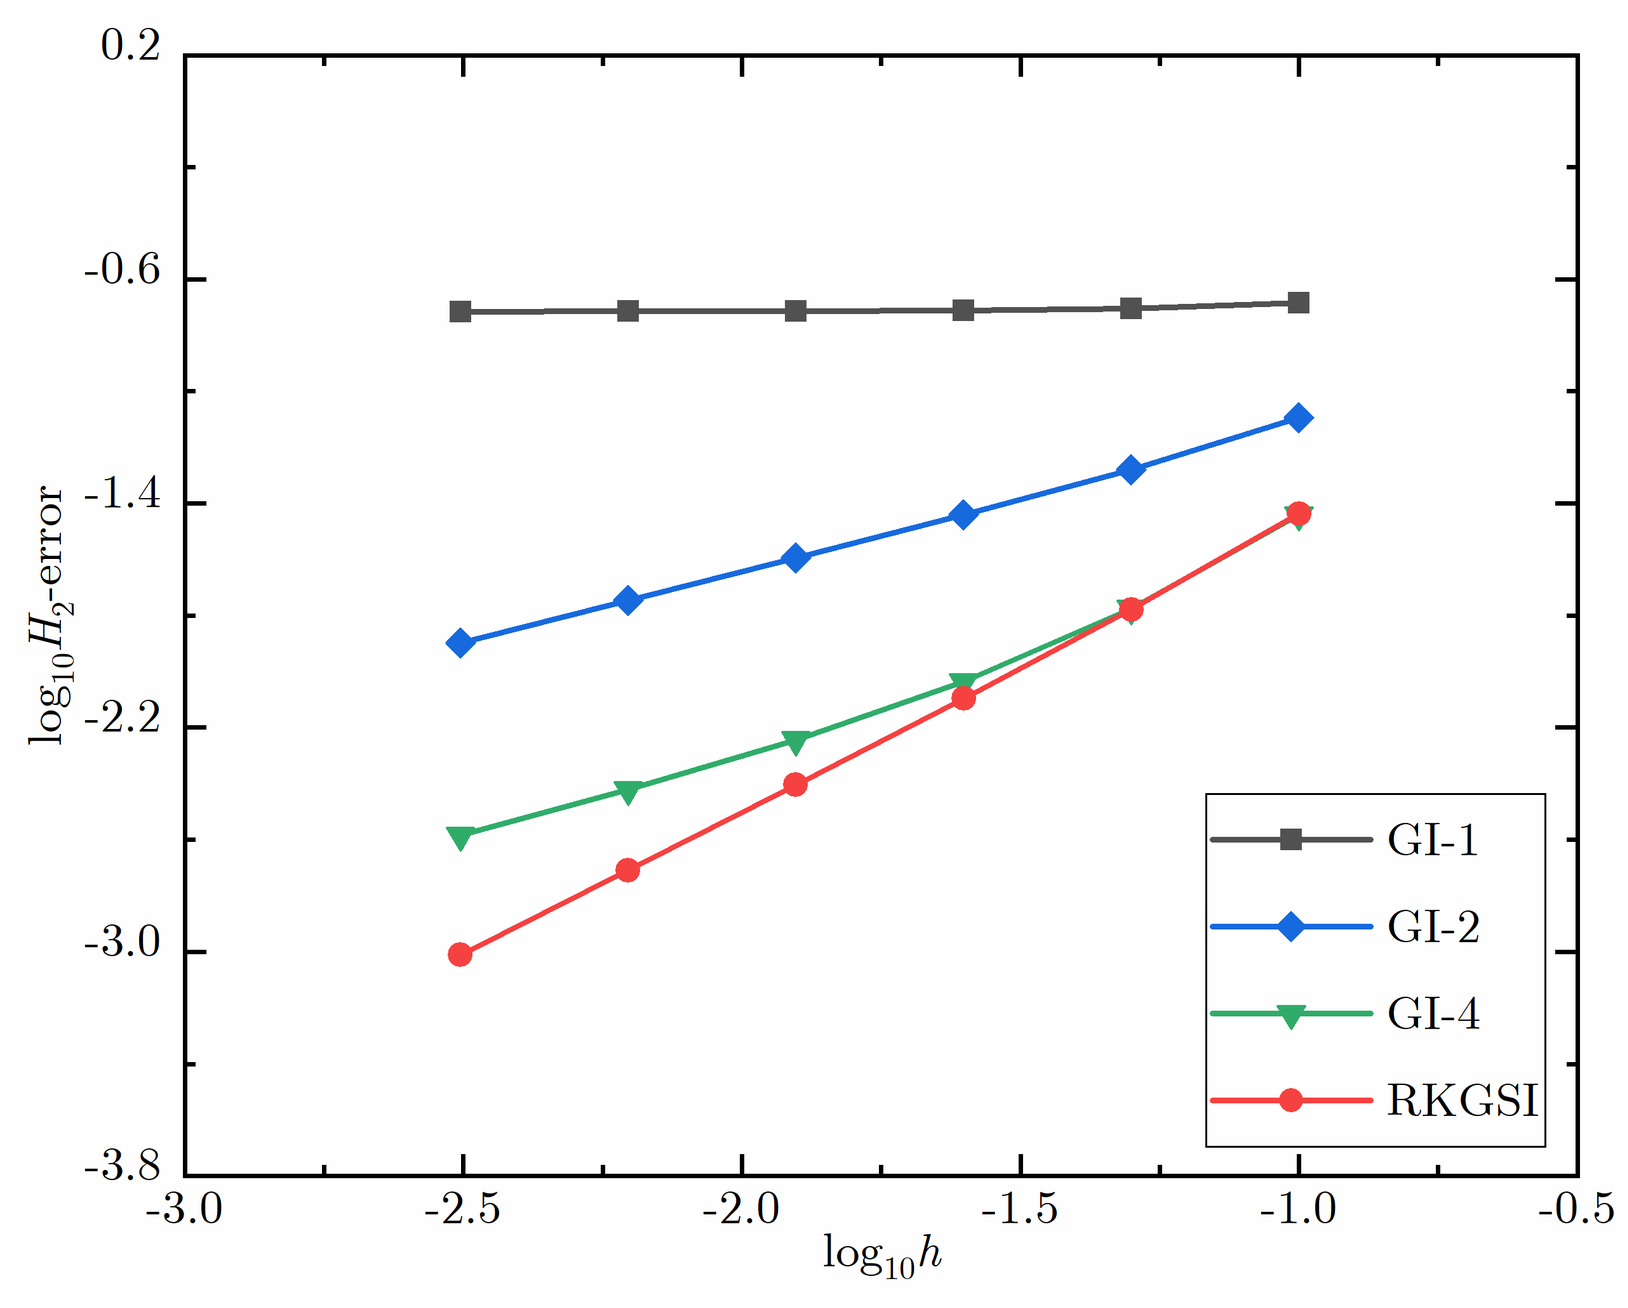
\includegraphics[width=0.55\textwidth]{figs/fig08.png}
\caption{$H_2$-error comparison for the 1D cantilever beam with $p=2$.}\label{fig:8}
\end{figure}

Figs. \ref{fig:6}--\ref{fig:8} show the convergence rates of compute error regarding to $L_2$, $H_1$ and $H_2$ norm for Gauss integration based methods (GI-1, 2, 4) and reproducing kernel gradient smoothing integration based method (RKGSI).
It clearly evinces the importance of the order of basis function, when $p=2$, all the integral schemes both ensure second order of convergence for $L_2$ error even though RKGSI possess the same order of integration consistency as basis function ($q=p=2$), while the integration consistency of GI only be $q=1$.
For $H_1$ and $H_2$ error in Figs. \ref{fig:7} and \ref{fig:8}, notable advantages of RKGSI can be observed with smaller nodal distances, which originates from deficiency of integration consistency of GI.

Another 2D benchmark problem is a left-clamped plate shown in Fig. \ref{fig:9}, whose material properties is the same as the previous 1D beam, geometry property is $L_x=L_y=1$.
The analytical solution and boundary conditions are given by:
\begin{equation}\label{eq:91}
\begin{cases}
w=\left(\sin x-x\right)\left(y+y^{2}\right)\\[2pt]
w(0,y)=0,\quad \theta(0,y)=0
\end{cases}
\end{equation}

\begin{figure}[pos=htbp]
\centering
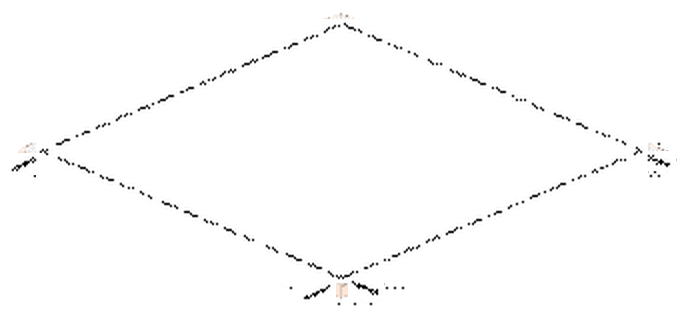
\includegraphics[width=0.6\textwidth]{figs/fig09.png}
\caption{Description of left-clamped plate.}\label{fig:9}
\end{figure}

\begin{figure}[pos=htbp]
\centering
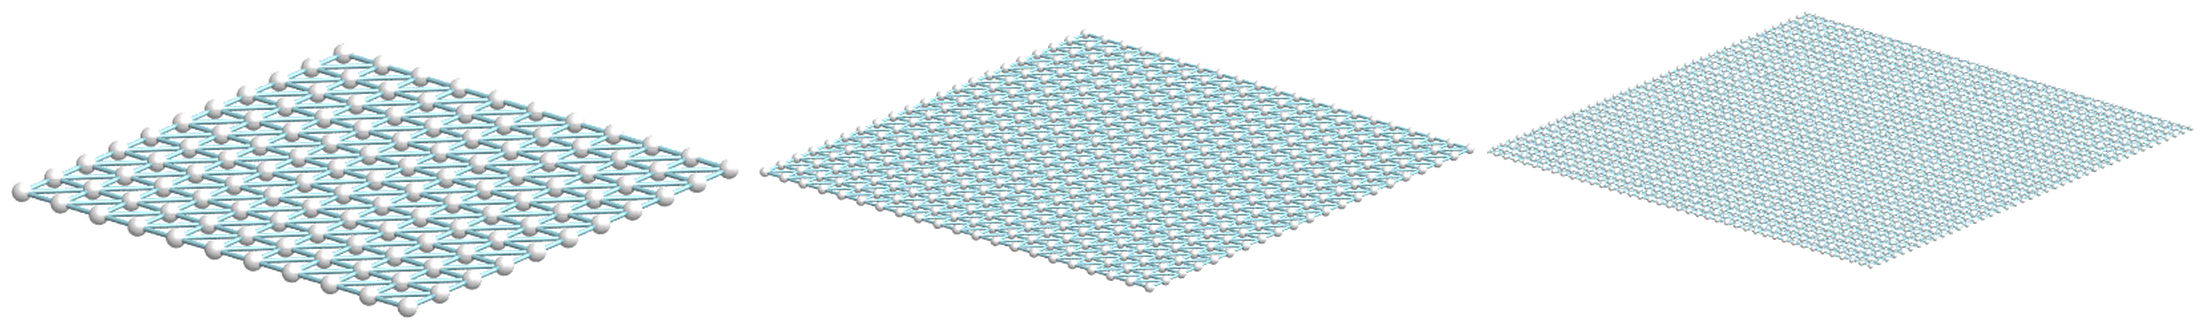
\includegraphics[width=\textwidth]{figs/fig10.png}
\caption{Meshfree discretizations with 36, 121, 441 nodes.}\label{fig:10}
\end{figure}

The normalized support size for quadratic meshfree formulation is set as 2.6.
As shown in Fig. \ref{fig:10}, five regular meshfree discretizations with 36, 121, 441, 1681, 6561 nodes are employed in order to observe the numerical convergence rates of GI and RKGSI.
The convergence performances listed in Figs. \ref{fig:11}--\ref{fig:13} further confirm the theoretical conclusion, which is, when $p=2$, the $L_2$, $H_1$ and $H_2$ errors of RKGSI with $q=p$ respectively converge at the rate of 2, 2 and 1 under refining discretizations, while the convergence rates of GI only achieves about 2, 1 and 0 due to a smaller order of integration consistency than basis function ($q<p$) in traditional Galerkin meshfree methods (such as GI-3, 6 and 9).

\begin{figure}[pos=htbp]
\centering
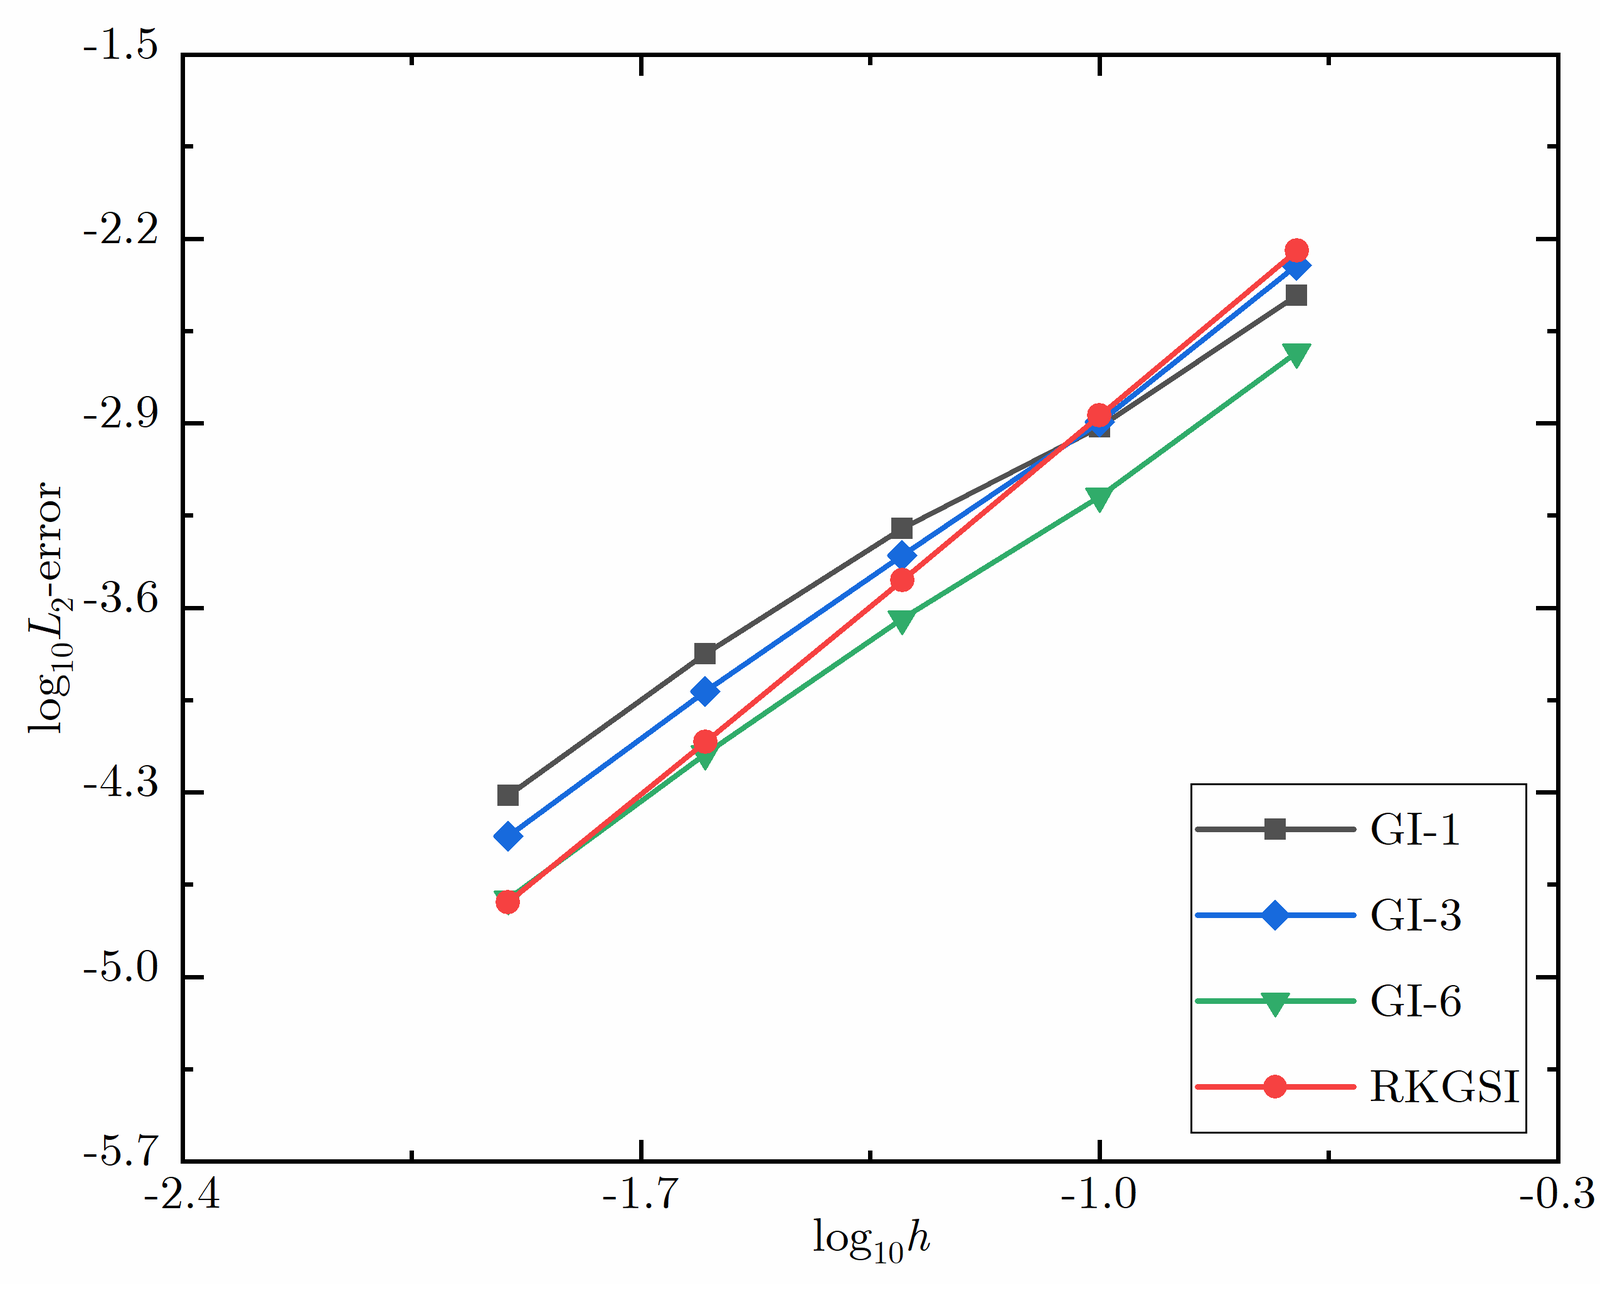
\includegraphics[width=0.55\textwidth]{figs/fig11.png}
\caption{$L_2$-error comparison for the 2D singly clamped plate with $p=2$.}\label{fig:11}
\end{figure}

\begin{figure}[pos=htbp]
\centering
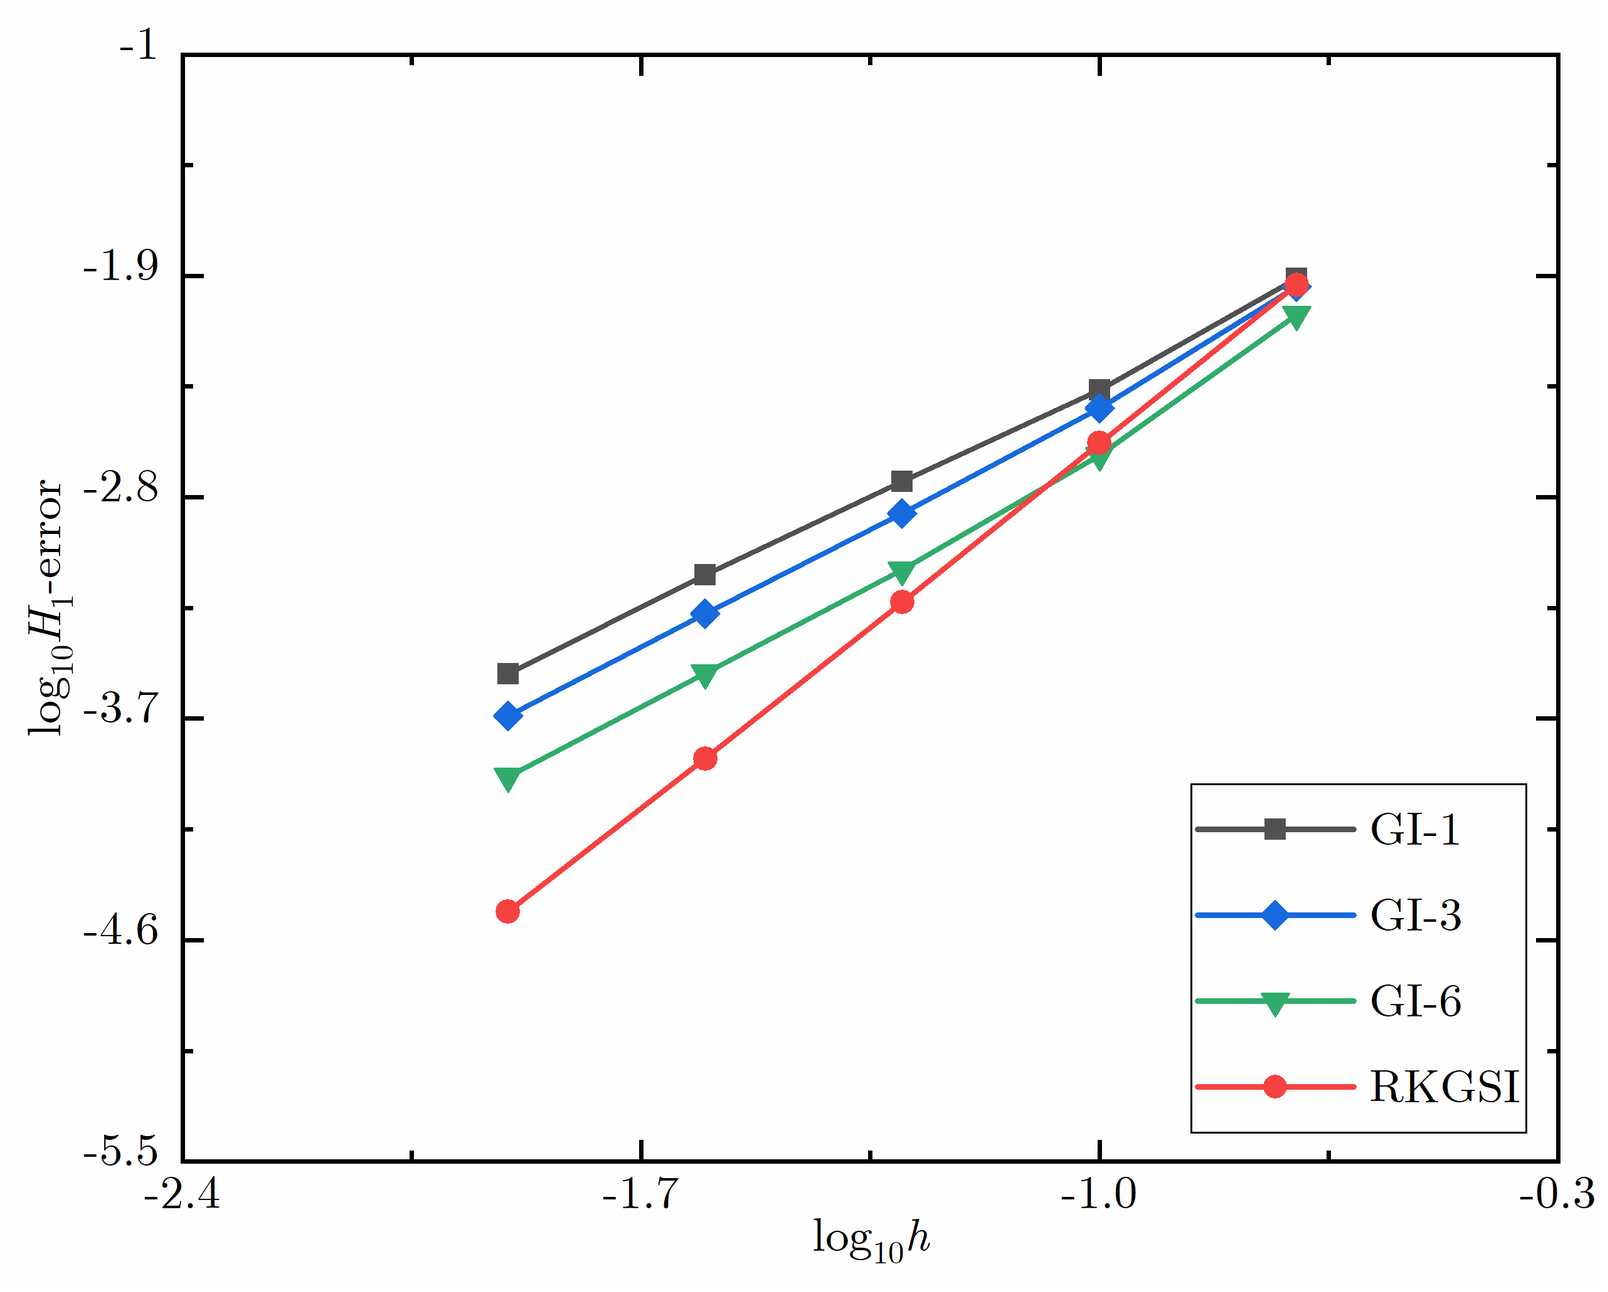
\includegraphics[width=0.55\textwidth]{figs/fig12.png}
\caption{$H_1$-error comparison for the 2D singly clamped plate with $p=2$.}\label{fig:12}
\end{figure}

\begin{figure}[pos=htbp]
\centering
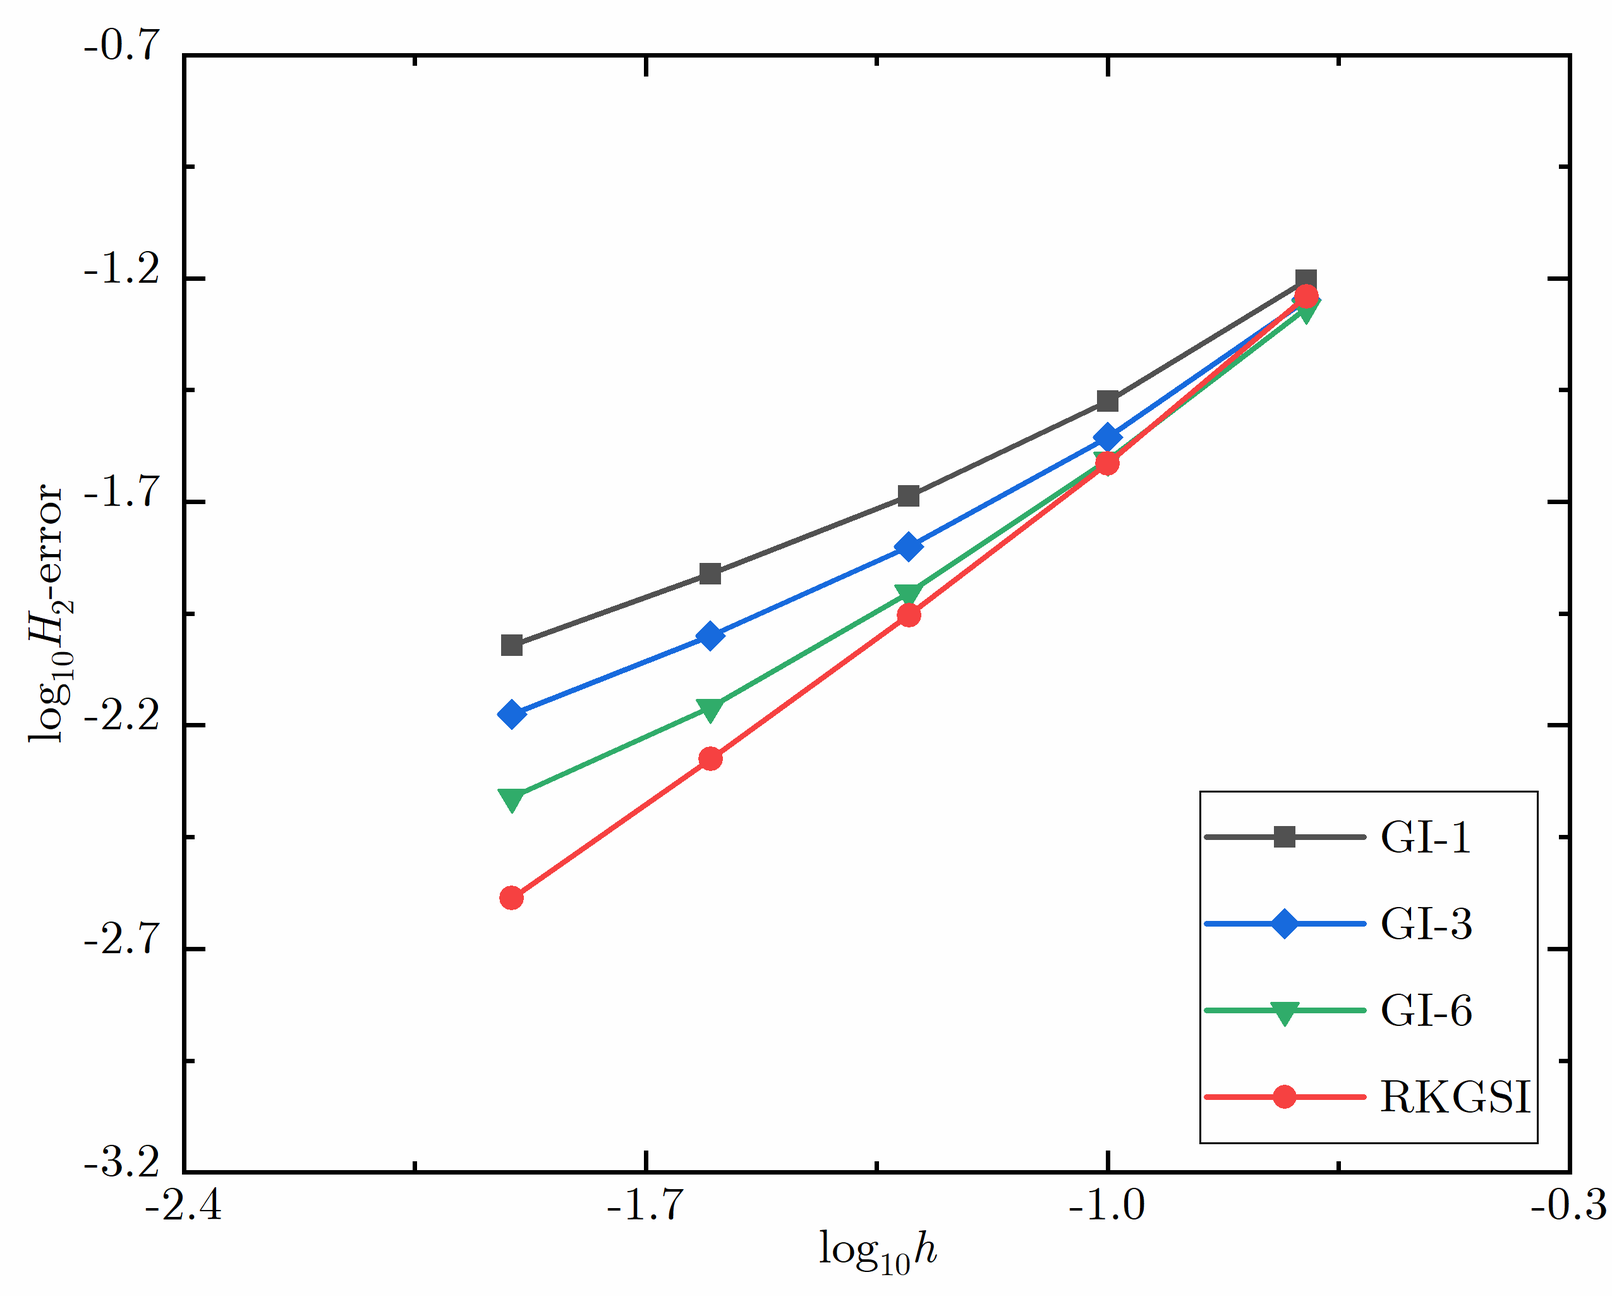
\includegraphics[width=0.55\textwidth]{figs/fig13.png}
\caption{$H_2$-error comparison for the 2D singly clamped plate with $p=2$.}\label{fig:13}
\end{figure}

For better illustrating the importance of integration consistency, in subsequent contents, we will focus on cubic and quartic meshfree formulation with GI and RGKSI.

\subsection{1D manufactured beam}\label{sec:manufactured1d}

In order to assess the convergence performance of Galerkin meshfree methods with cubic and quartic basis function, we consider a manufactured beam as shown in Fig. \ref{fig:14}, and an octal polynomial solution is employed to perform the meshfree computation:
\begin{equation}\label{eq:92}
w=x^{8}/100+2x^{7}/100+x^{6}+x^{5}+5x^{4}+3x^{3}+4x^{2}+5x+6
\end{equation}
All specific values of boundary conditions are determined by Eq. \eqref{eq:92}.
The displacement and moment boundary conditions are imposed on both sides.
Also, the material and geometry properties are the same as 1D cantilever beam in Section \ref{sec:quadratic}.

\begin{figure}[pos=htbp]
\centering
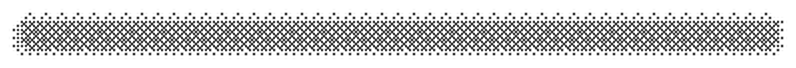
\includegraphics[width=0.85\textwidth]{figs/fig14.png}
\caption{Description of 1D manufactured beam.}\label{fig:14}
\end{figure}

Five meshfree discretizations with 11, 21, 41, 81, 161 nodes are adopted to observe the convergence performance.
For meshfree computation, the normalized support sizes are respectively prescribed as 3.5 and 4.5 for $p=3,4$.
The convergence results referring to $L_2$, $H_1$ and $H_2$ error norms for cubic and quartic meshfree formulation are listed in Figs. \ref{fig:15}--\ref{fig:20}, respectively.
The results clearly show that the convergence rates of GI-3, GI-6 and GI-9 adopted in cubic meshfree formulation, GI-4, GI-8 and GI-13 adopted in quartic meshfree formulation both are 2, 1, 0, respectively.
This is because Gauss integration can not meet the cubic and quartic integration constraints corresponding to the orders of basis functions, i.e., the integration consistency of GI is $q=1$, which is lower than $p$, thus the integration error totally governs the convergence performance of Galerkin meshfree methods with the nodal distance constantly decreasing.
On the contrary, according to the previous description, since RKGSI based meshfree formulation possess corresponding integration consistency $q=p$, it is capable for producing optimal convergence rates of $L_2$, $H_1$ and $H_2$ error norms, which respectively are 4, 3 and 2 in cubic case, 5, 4, 3 in quartic case.

\begin{figure}[pos=htbp]
\centering
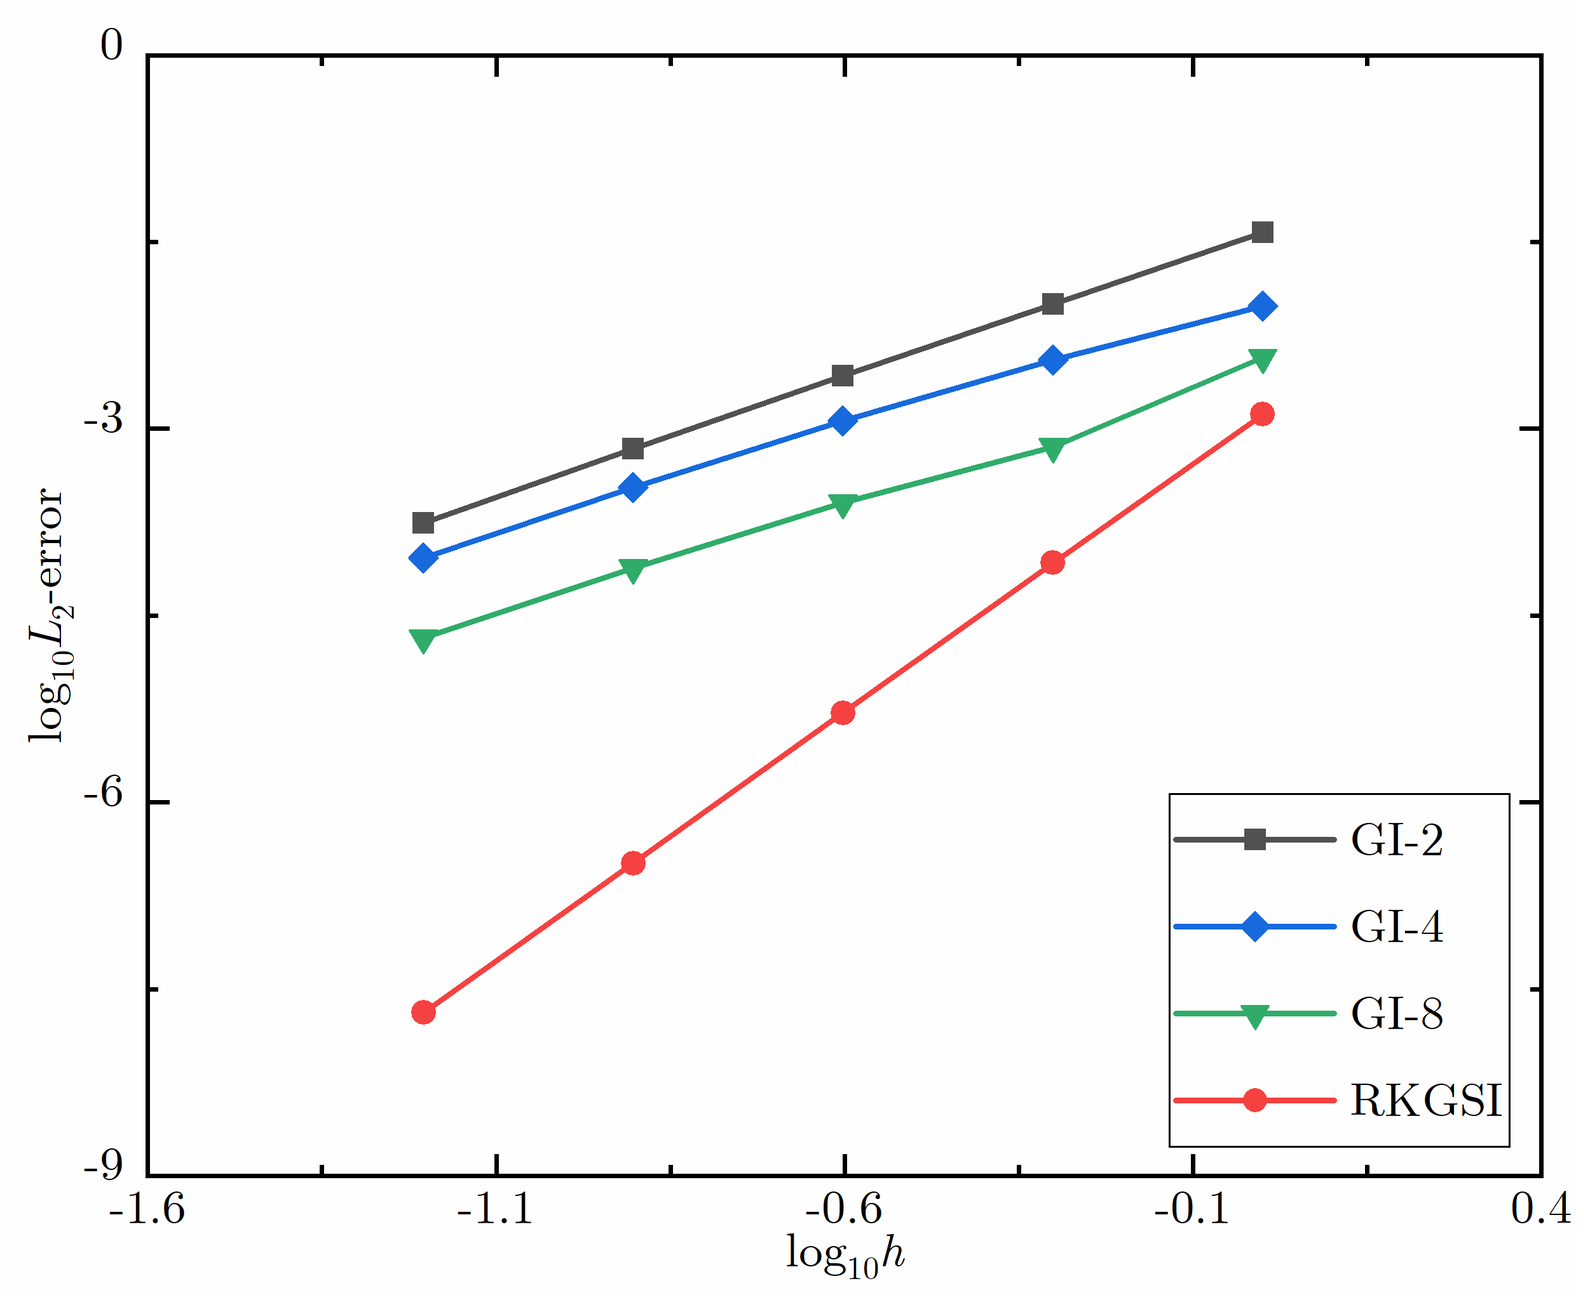
\includegraphics[width=0.55\textwidth]{figs/fig15.png}
\caption{$L_2$-error comparison for the 1D manufactured beam with $p=3$.}\label{fig:15}
\end{figure}

\begin{figure}[pos=htbp]
\centering
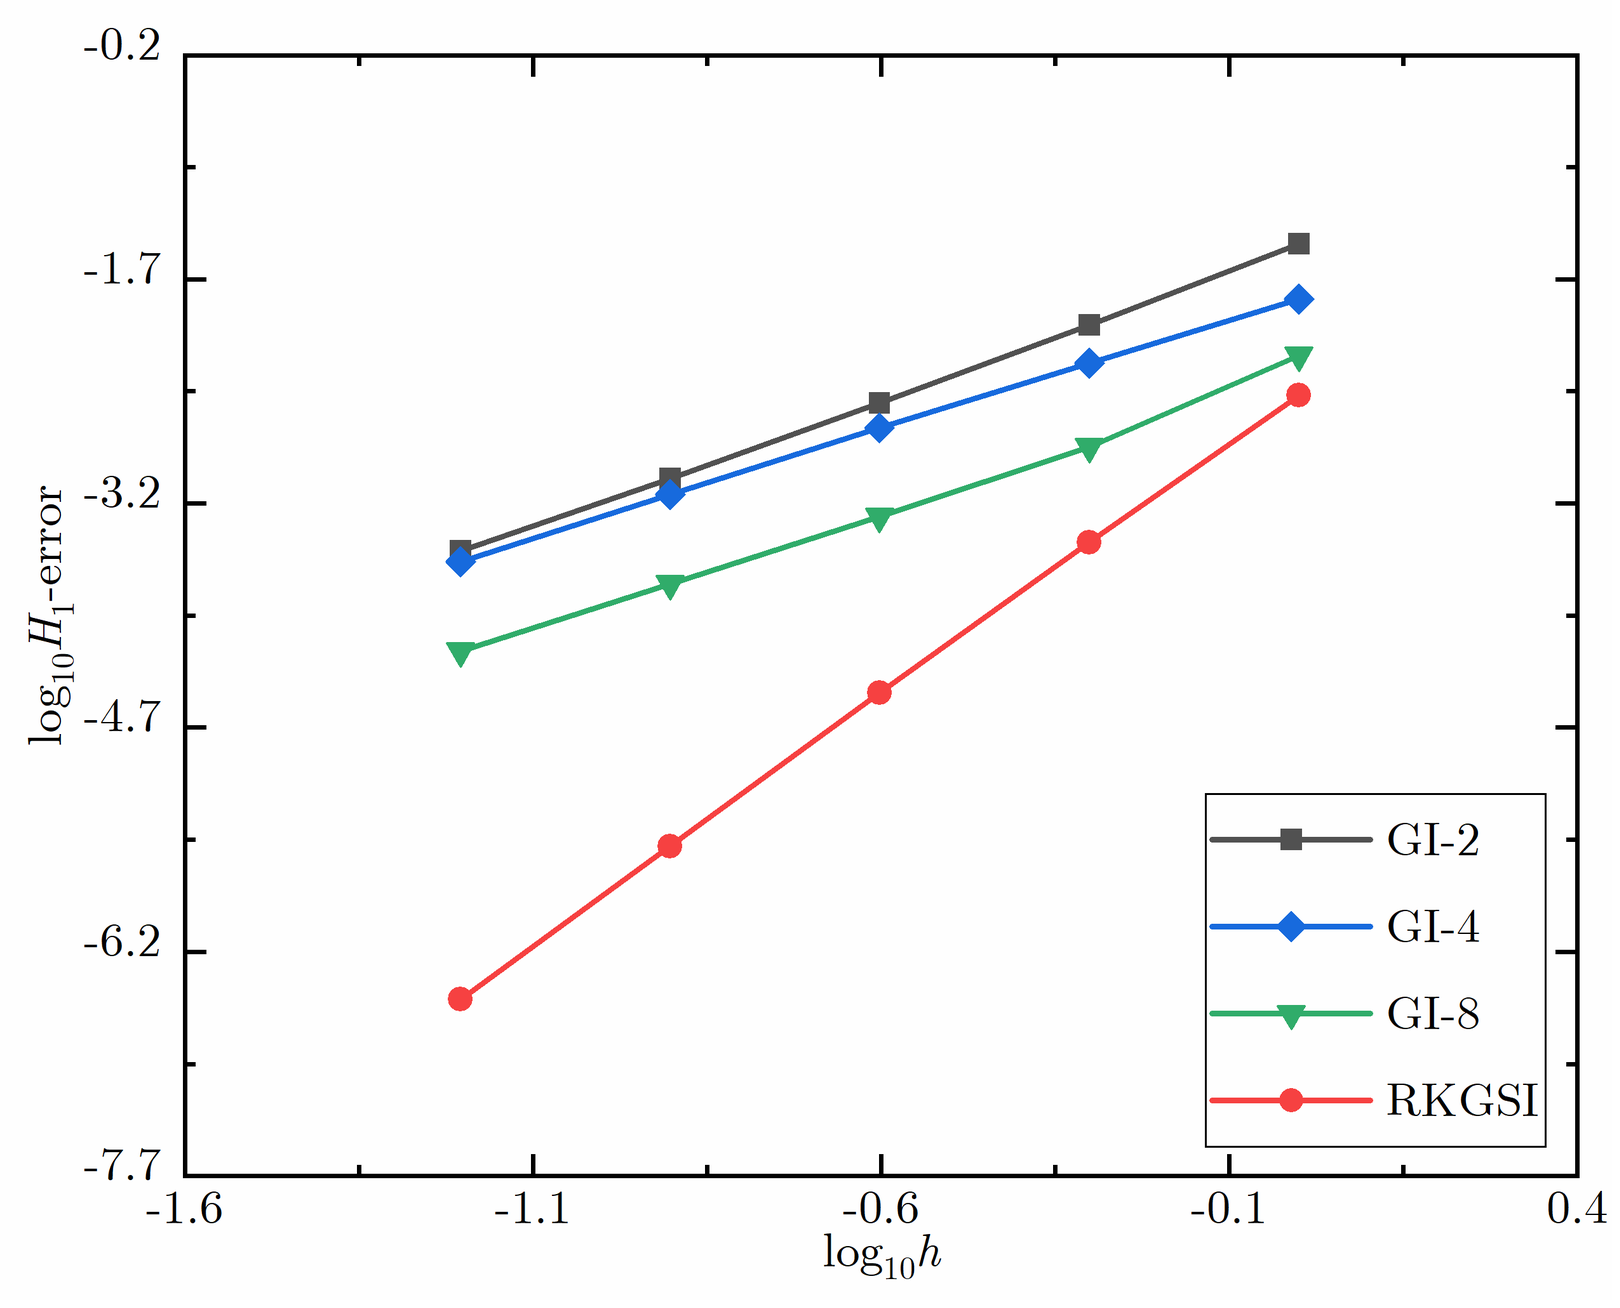
\includegraphics[width=0.55\textwidth]{figs/fig16.png}
\caption{$H_1$-error comparison for the 1D manufactured beam with $p=3$.}\label{fig:16}
\end{figure}

\begin{figure}[pos=htbp]
\centering
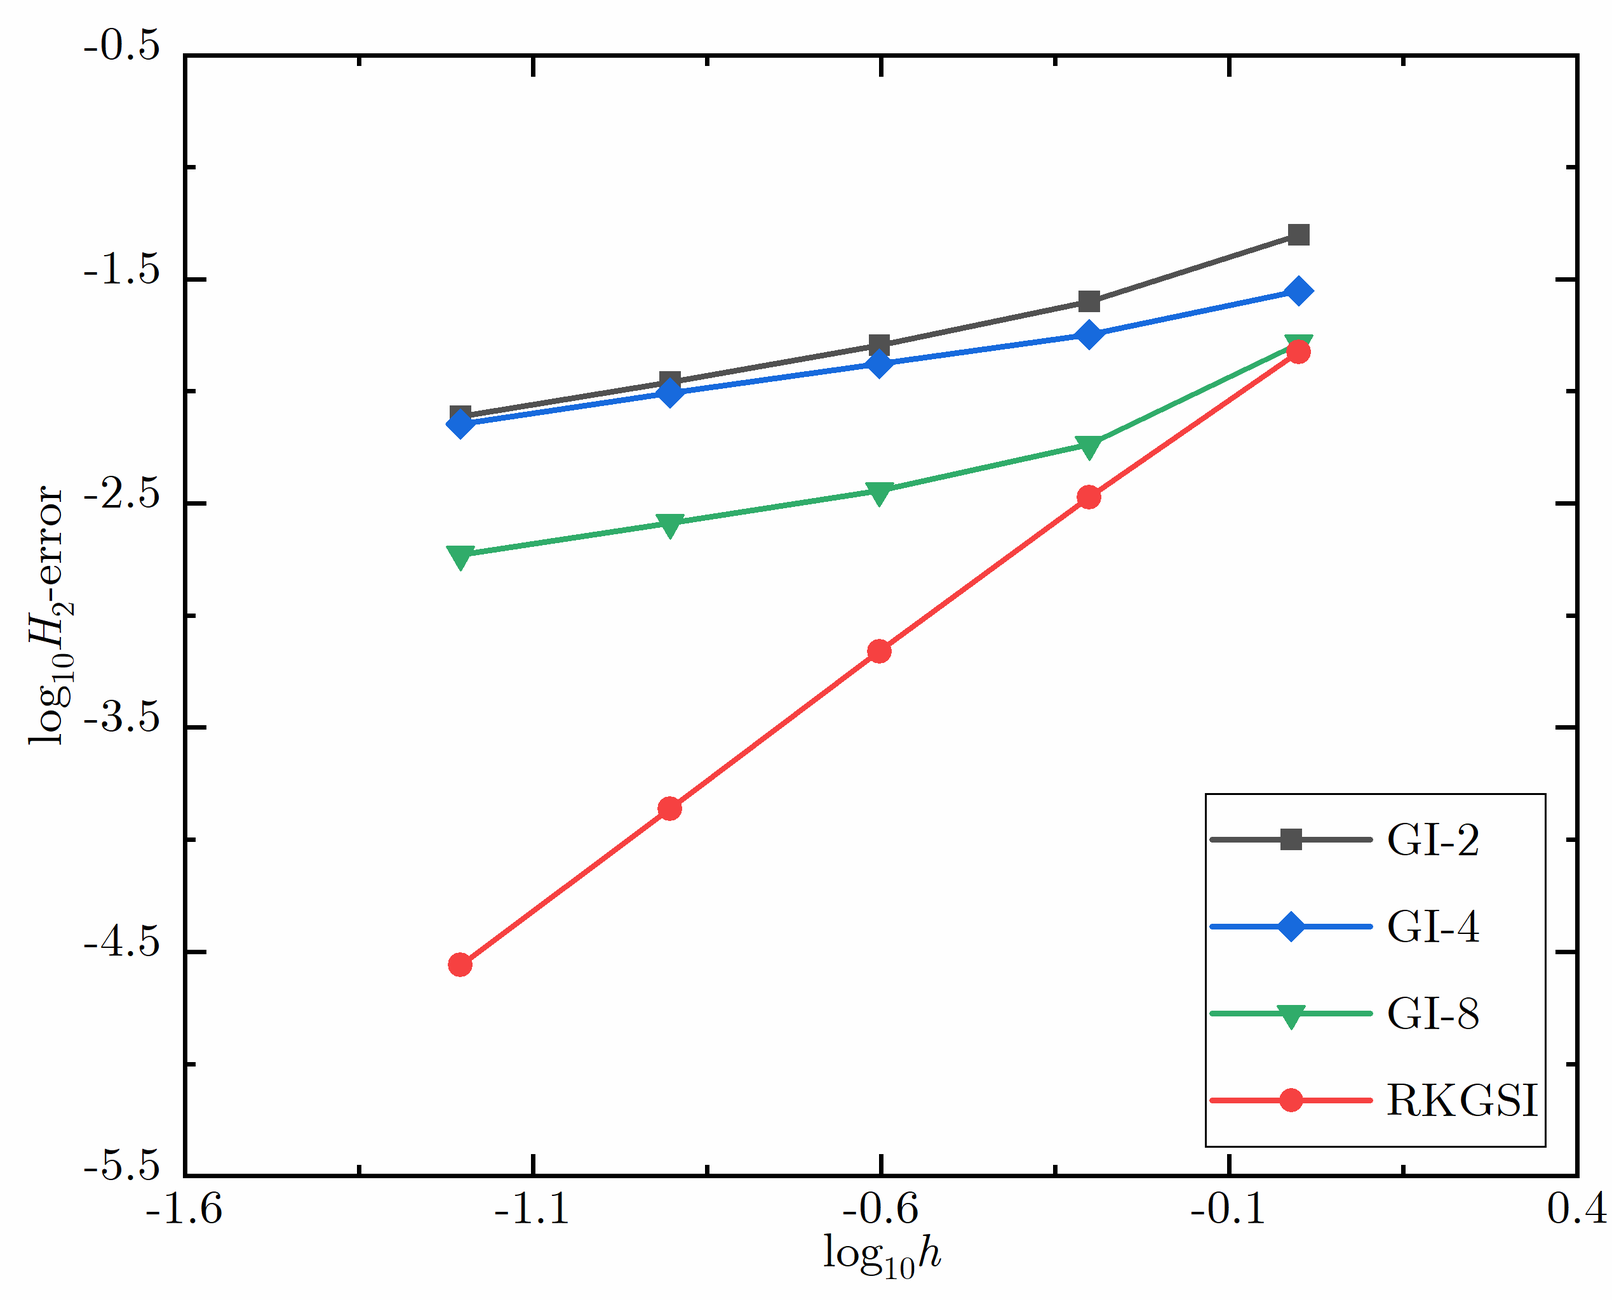
\includegraphics[width=0.55\textwidth]{figs/fig17.png}
\caption{$H_2$-error comparison for the 1D manufactured beam with $p=3$.}\label{fig:17}
\end{figure}

\begin{figure}[pos=htbp]
\centering
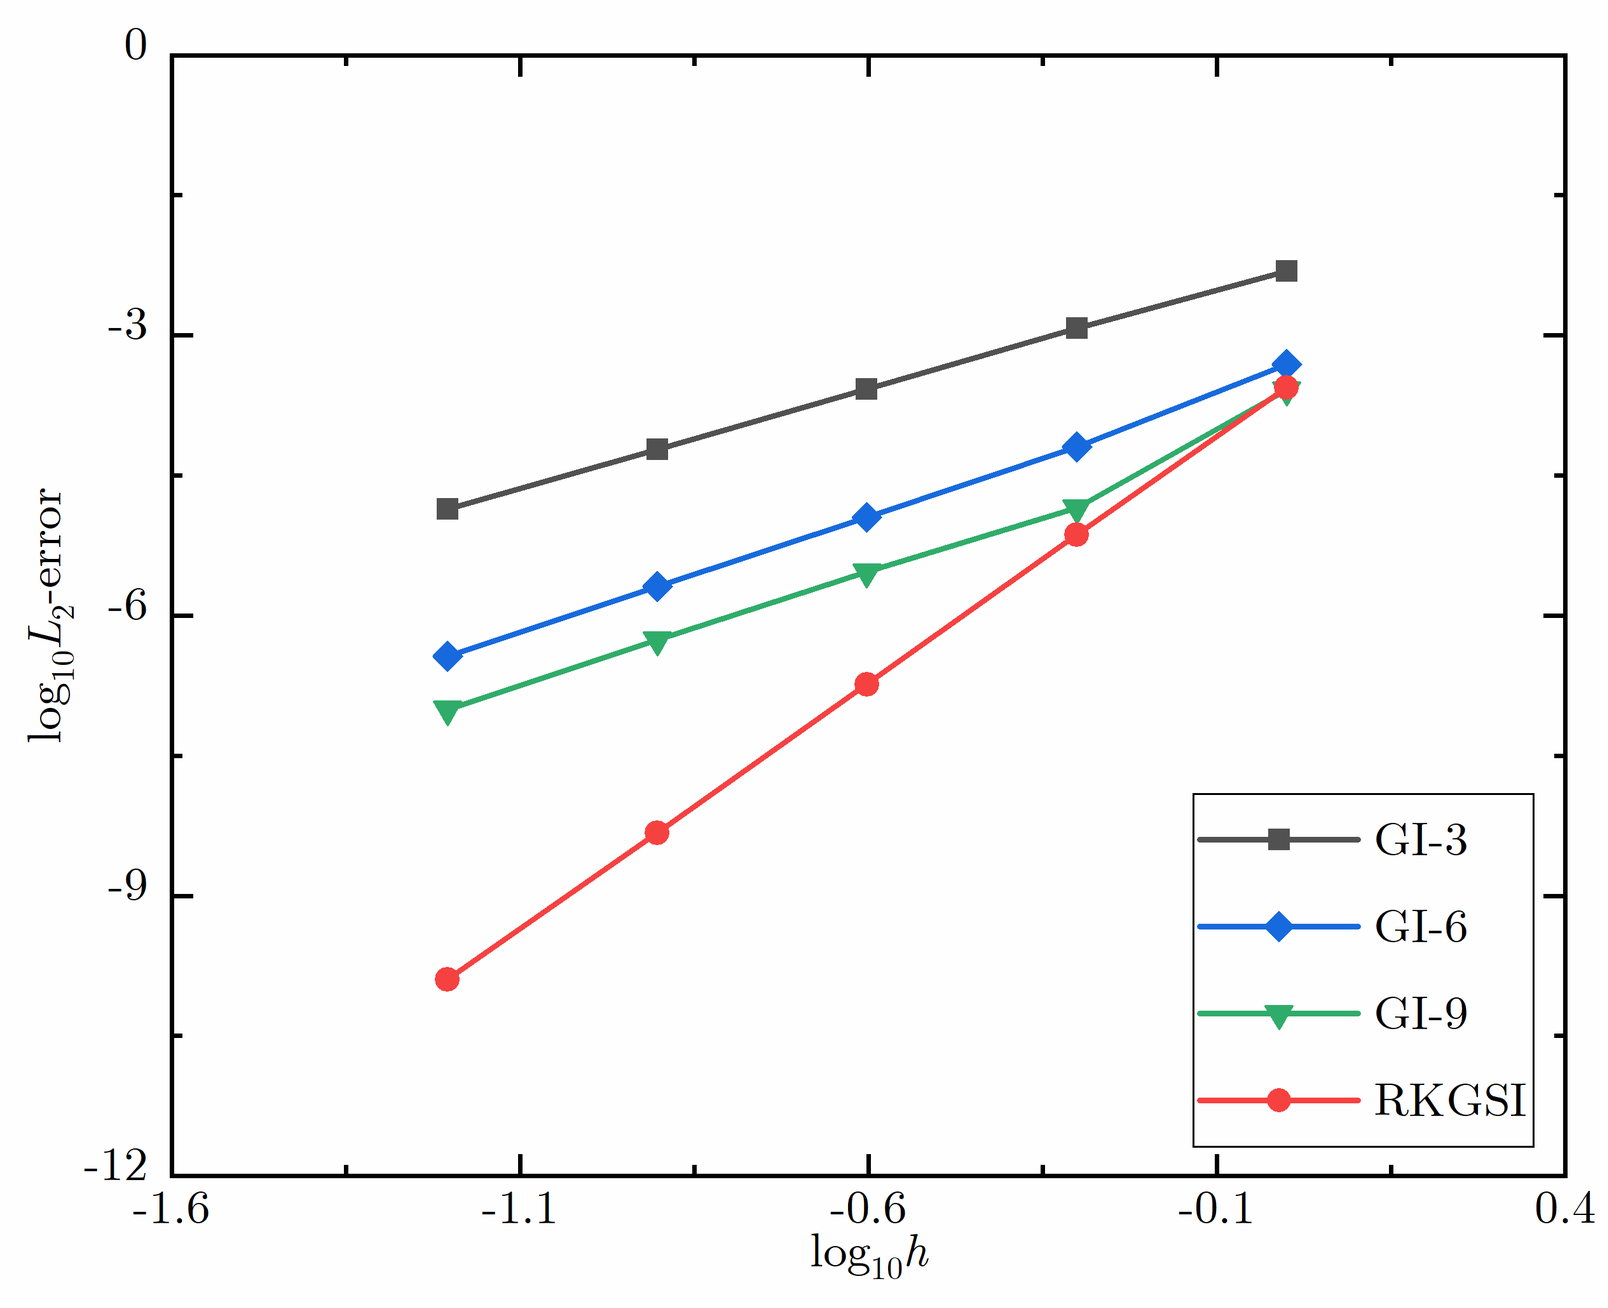
\includegraphics[width=0.55\textwidth]{figs/fig18.png}
\caption{$L_2$-error comparison for the 1D manufactured beam with $p=4$.}\label{fig:18}
\end{figure}

\begin{figure}[pos=htbp]
\centering
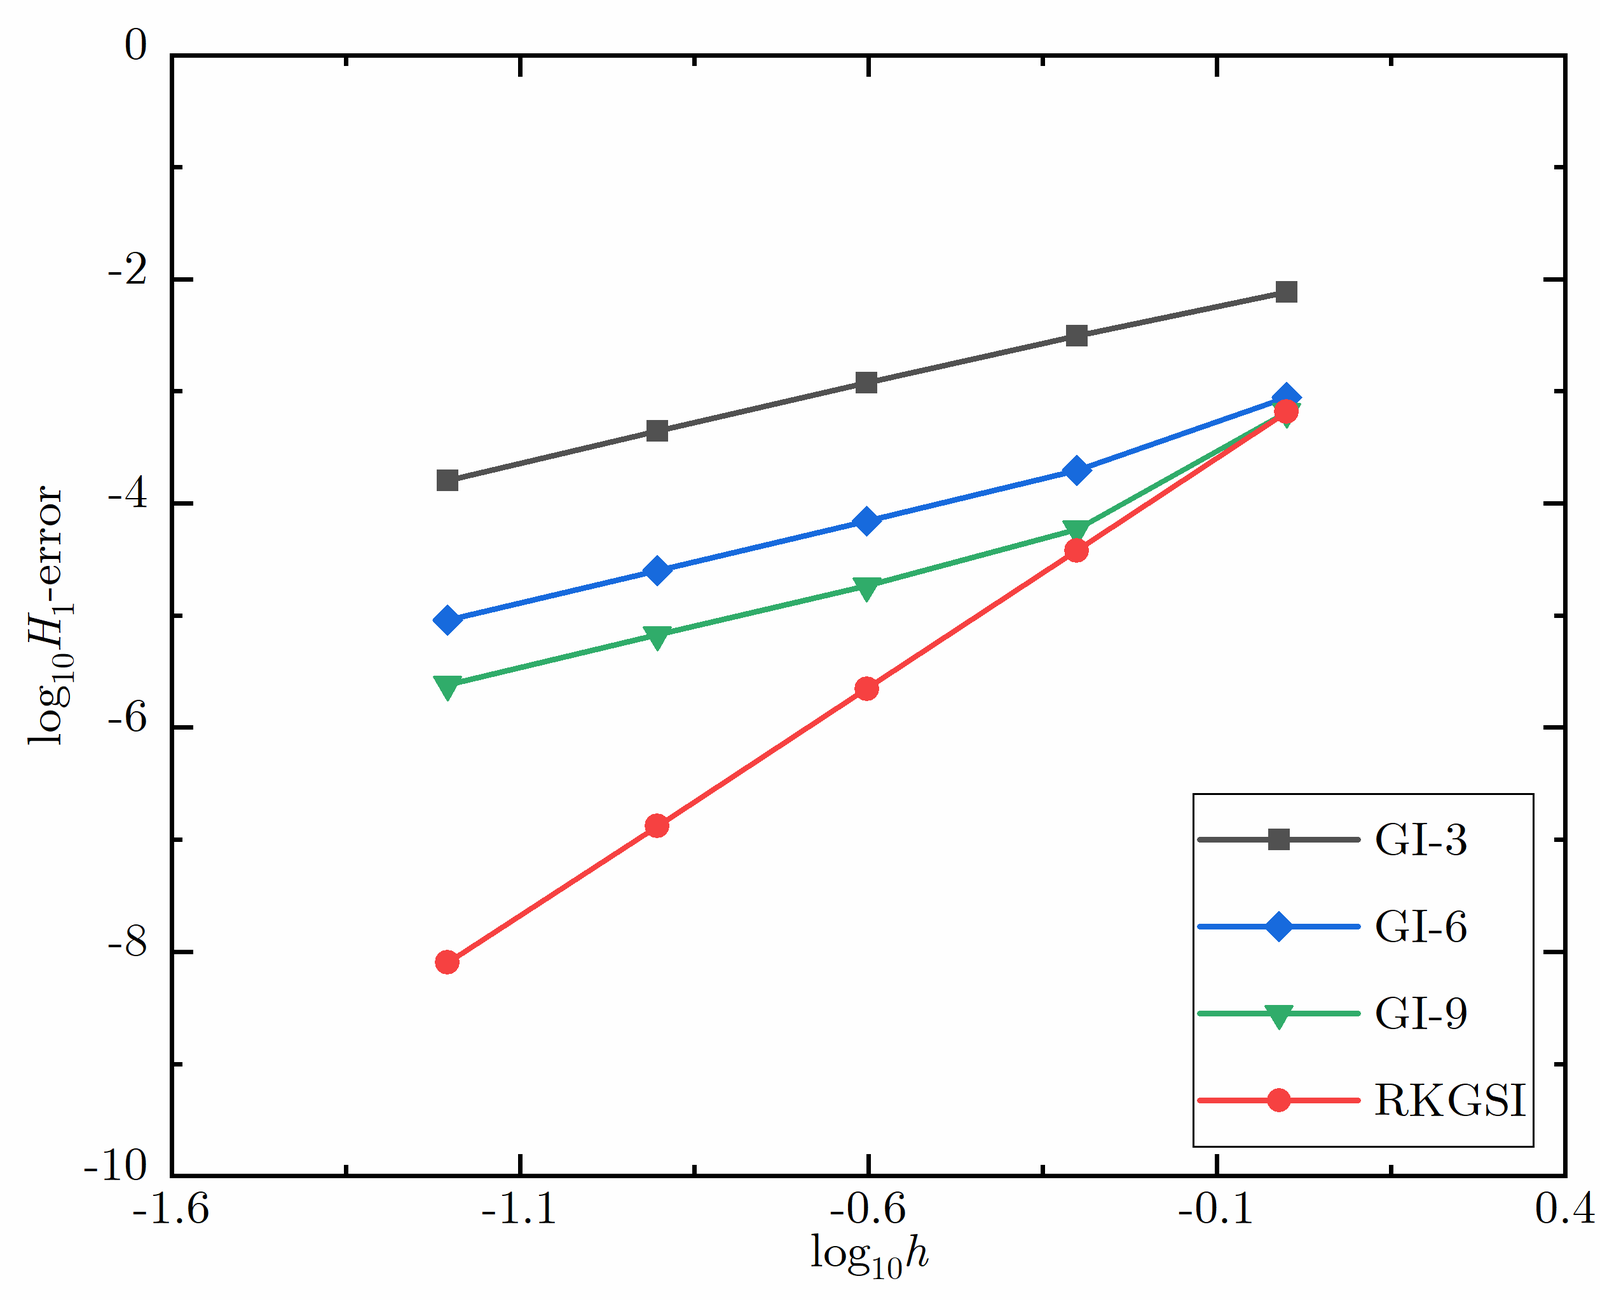
\includegraphics[width=0.55\textwidth]{figs/fig19.png}
\caption{$H_1$-error comparison for the 1D manufactured beam with $p=4$.}\label{fig:19}
\end{figure}

\begin{figure}[pos=htbp]
\centering
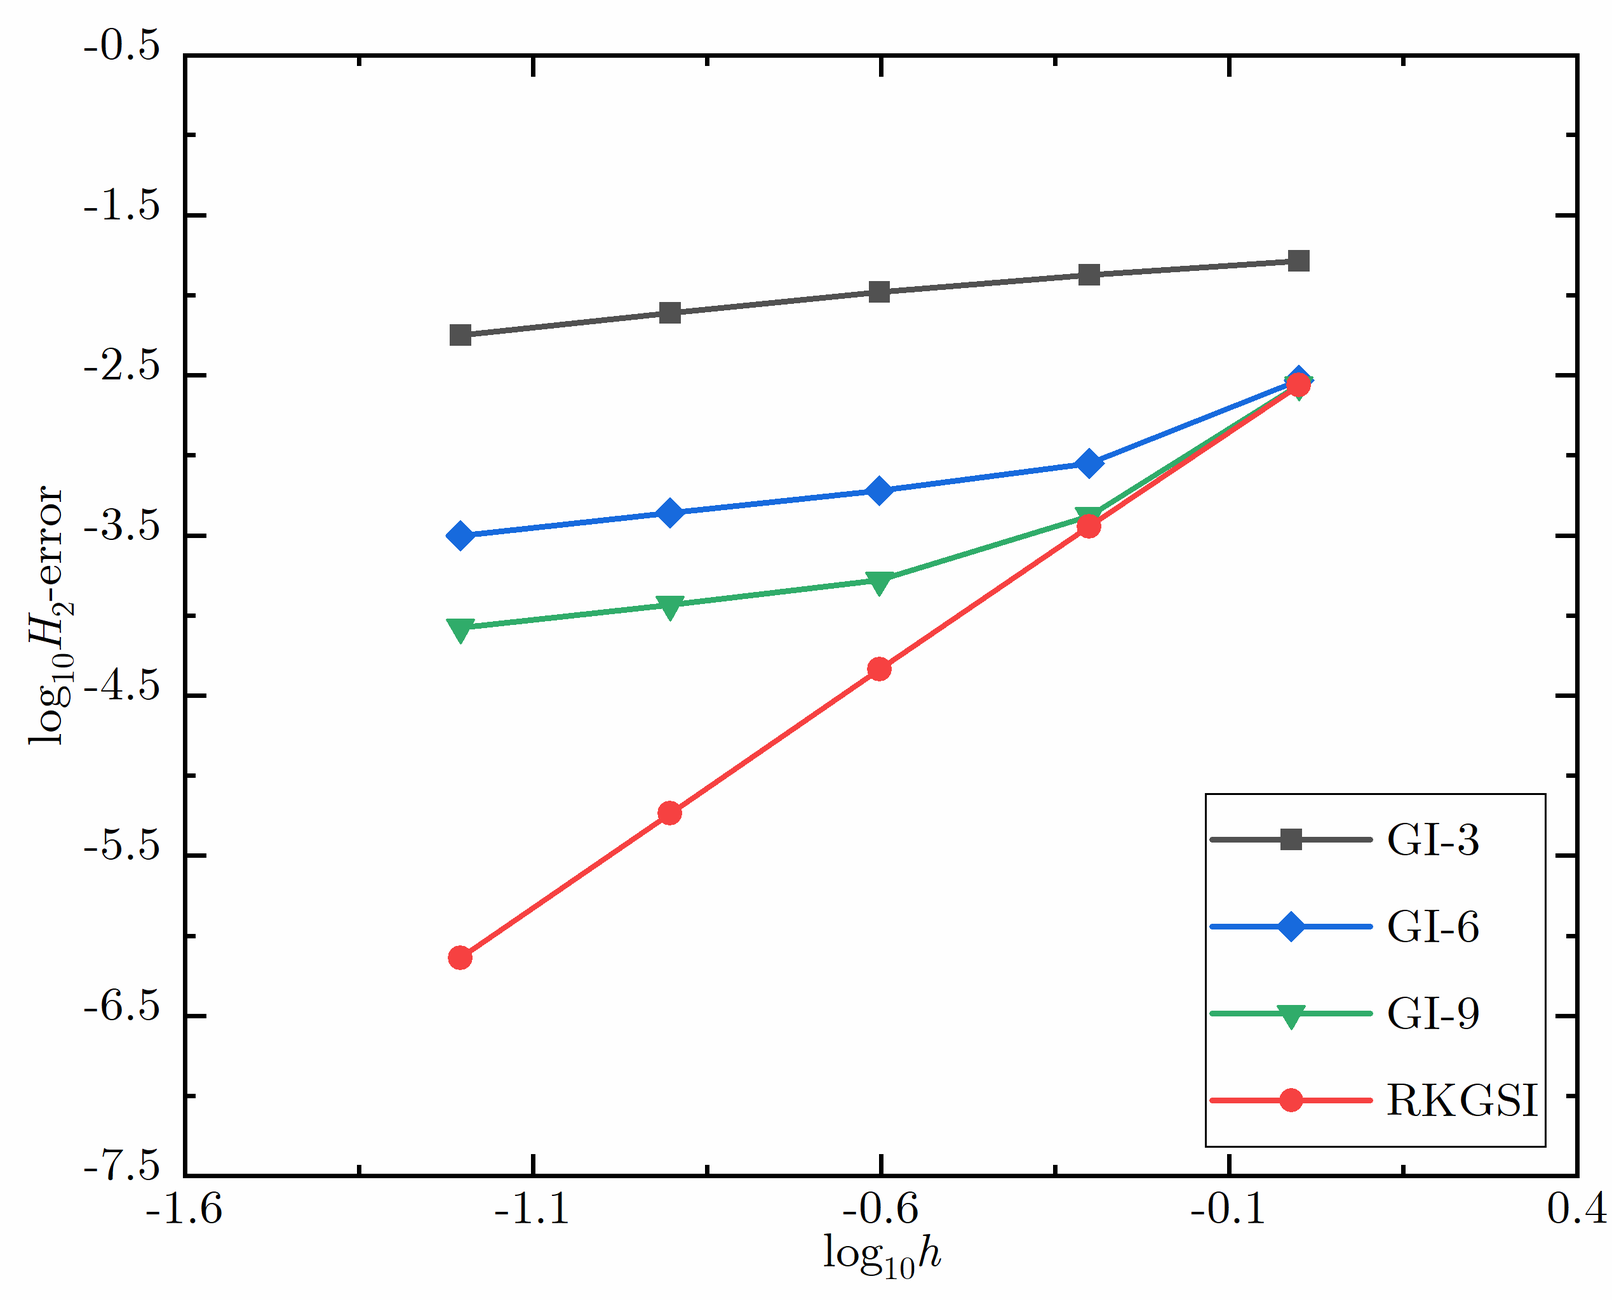
\includegraphics[width=0.55\textwidth]{figs/fig20.png}
\caption{$H_2$-error comparison for the 1D manufactured beam with $p=4$.}\label{fig:20}
\end{figure}

\subsection{2D manufactured plate}\label{sec:manufactured2d}

As shown in Fig. \ref{fig:21}, we perform the assessment of convergence performance on a manufactured plate, whose material and geometric properties are $D=2\times10^{4}$, Poisson's ratio $\nu=0.3$, length $L=10$.
The manufactured solution is state as:
\begin{equation}\label{eq:93}
w=\left(x+2y+1\right)^{8}/1000
\end{equation}

\begin{figure}[pos=htbp]
\centering
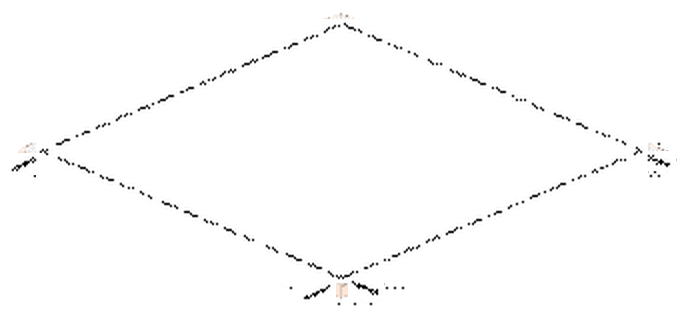
\includegraphics[width=0.6\textwidth]{figs/fig21.png}
\caption{Description of 2D manufactured plate.}\label{fig:21}
\end{figure}

The same as Section \ref{sec:quadratic}, five regular grids with 36, 121, 441, 1681, and 6561 nodes are applied to discrete the 2D domain.
The corresponding results are listed in Figs. \ref{fig:22}--\ref{fig:27}, which clearly evince that, with the reduce of nodal distance, the convergence rates of Gauss integration based method constantly deteriorate until reach the theoretical values, which are far below the optimal ones.
However, no matter which order of basis function is adopted, the convergence rates of RKGSI always keep $(p+1)$, $p$ and $(p-1)$, regarding the $L_2$, $H_1$ and $H_2$ error norms.

\begin{figure}[pos=htbp]
\centering
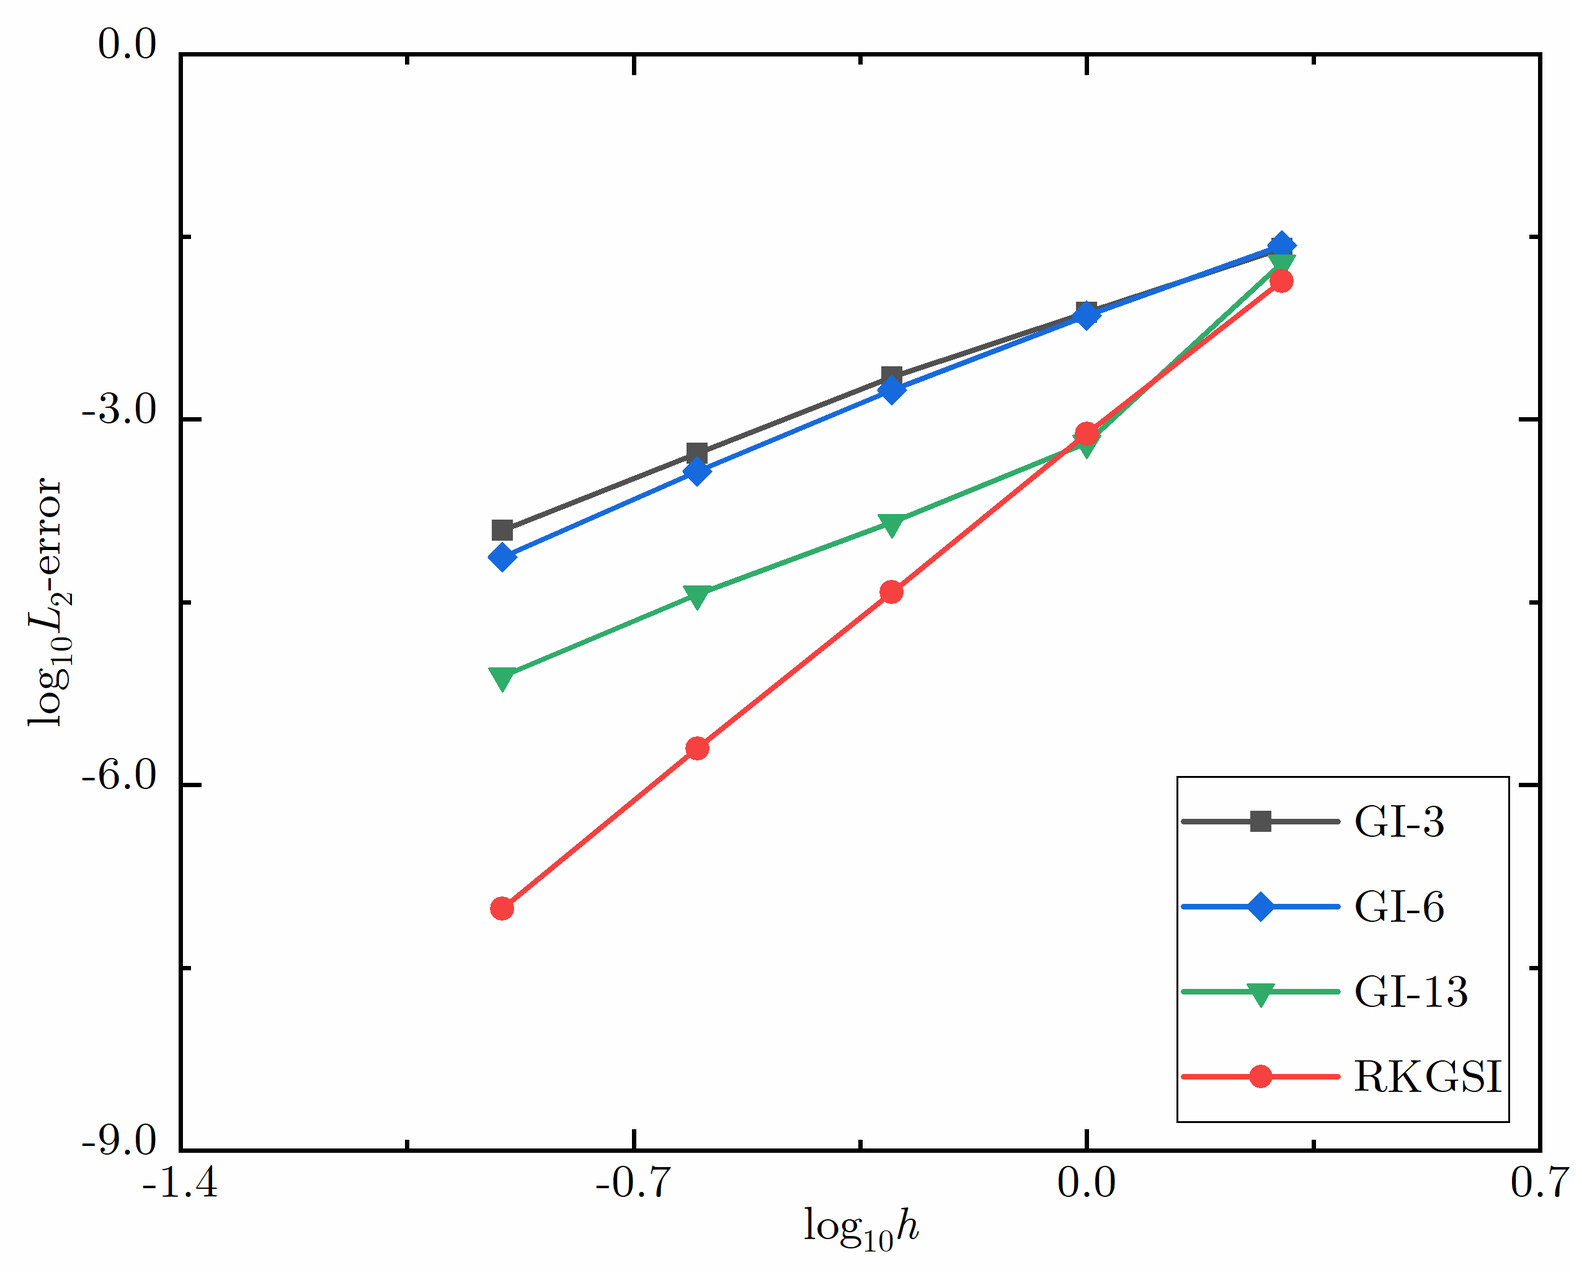
\includegraphics[width=0.55\textwidth]{figs/fig22.png}
\caption{$L_2$-error comparison for the 2D manufactured plate with $p=3$.}\label{fig:22}
\end{figure}

\begin{figure}[pos=htbp]
\centering
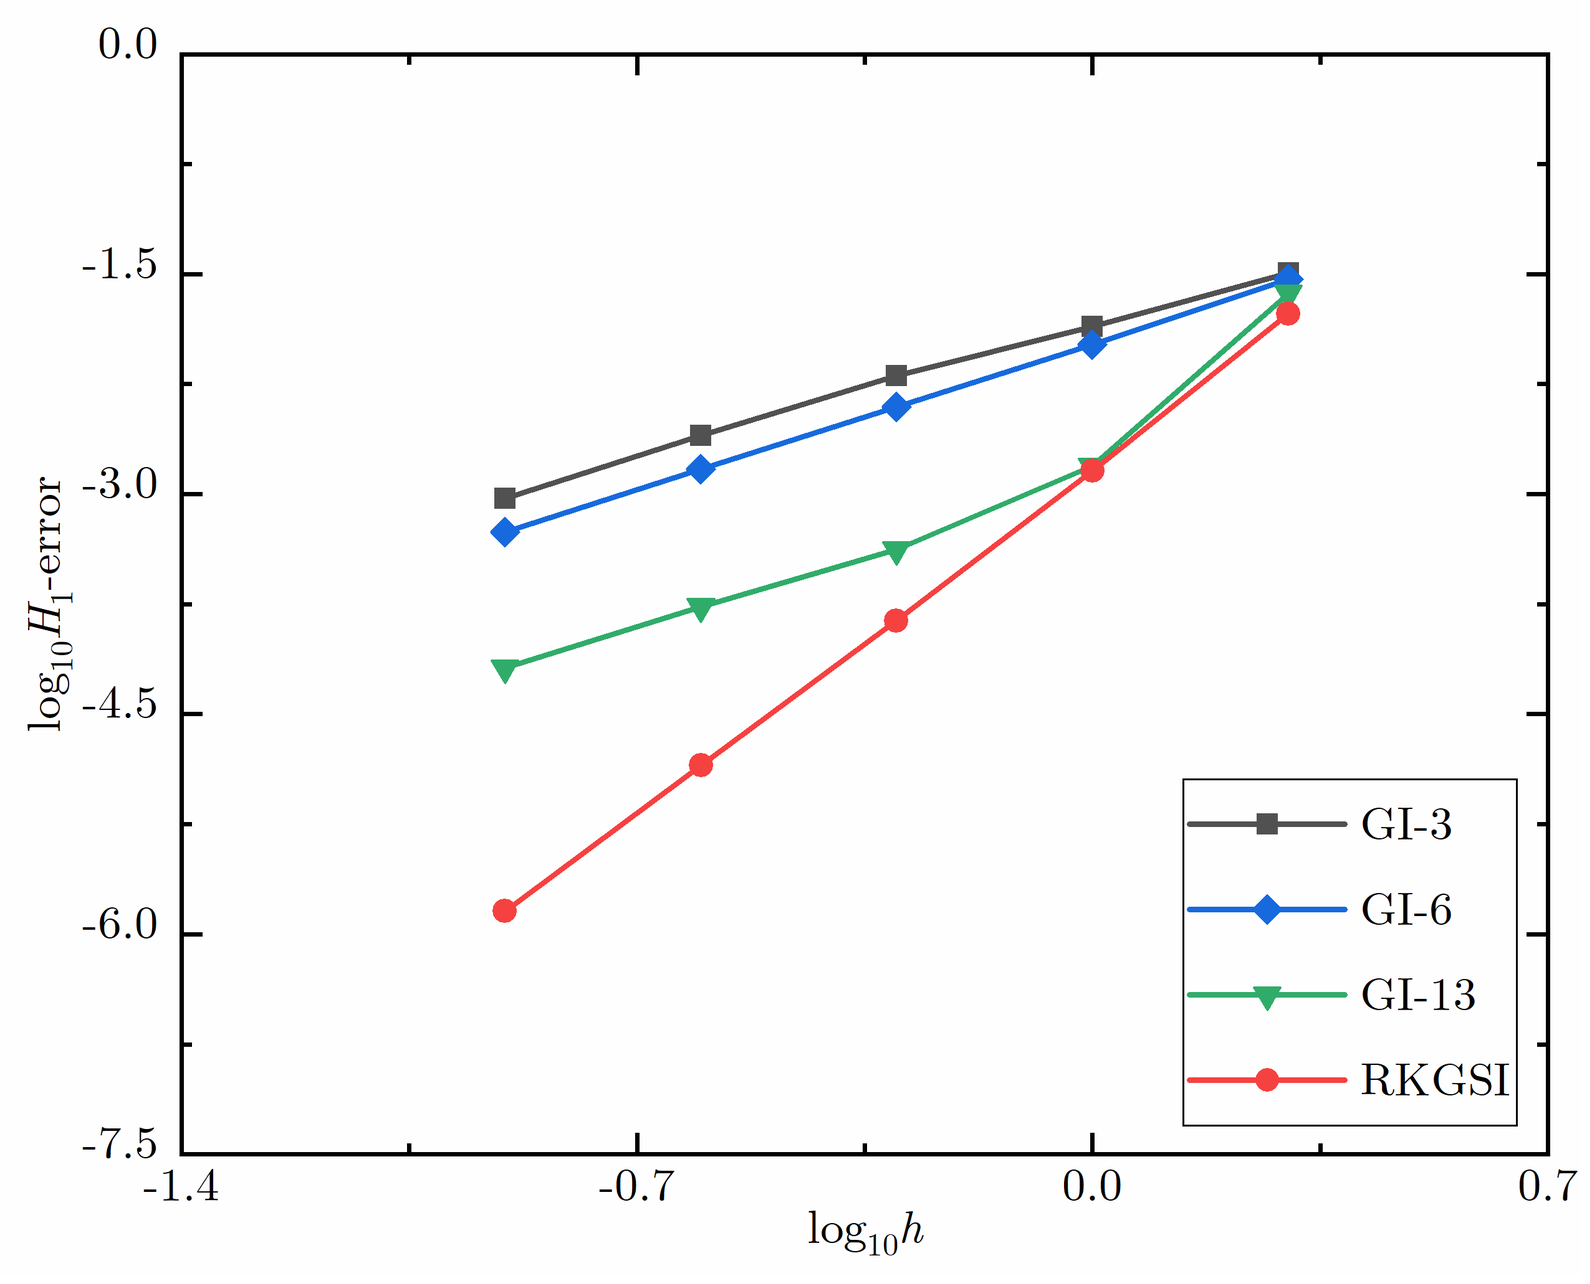
\includegraphics[width=0.55\textwidth]{figs/fig23.png}
\caption{$H_1$-error comparison for the 2D manufactured plate with $p=3$.}\label{fig:23}
\end{figure}

\begin{figure}[pos=htbp]
\centering
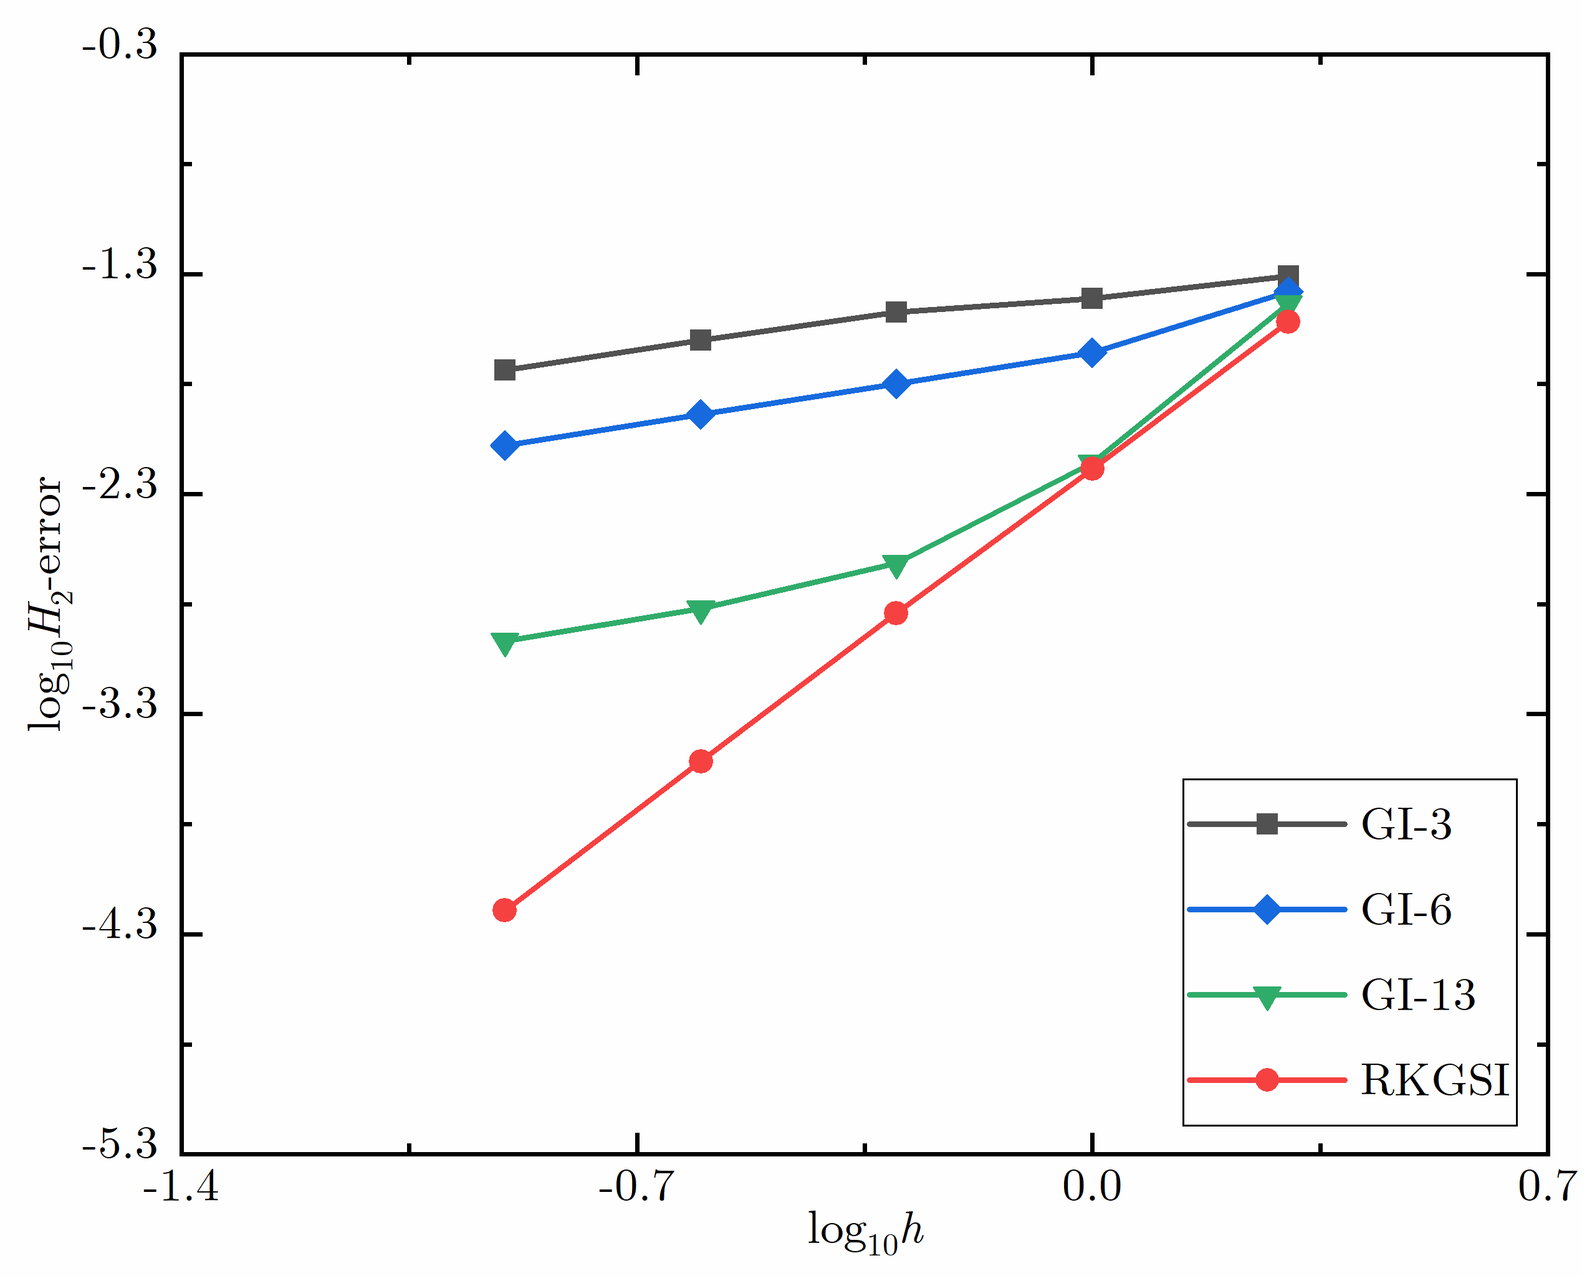
\includegraphics[width=0.55\textwidth]{figs/fig24.png}
\caption{$H_2$-error comparison for the 2D manufactured plate with $p=3$.}\label{fig:24}
\end{figure}

\begin{figure}[pos=htbp]
\centering
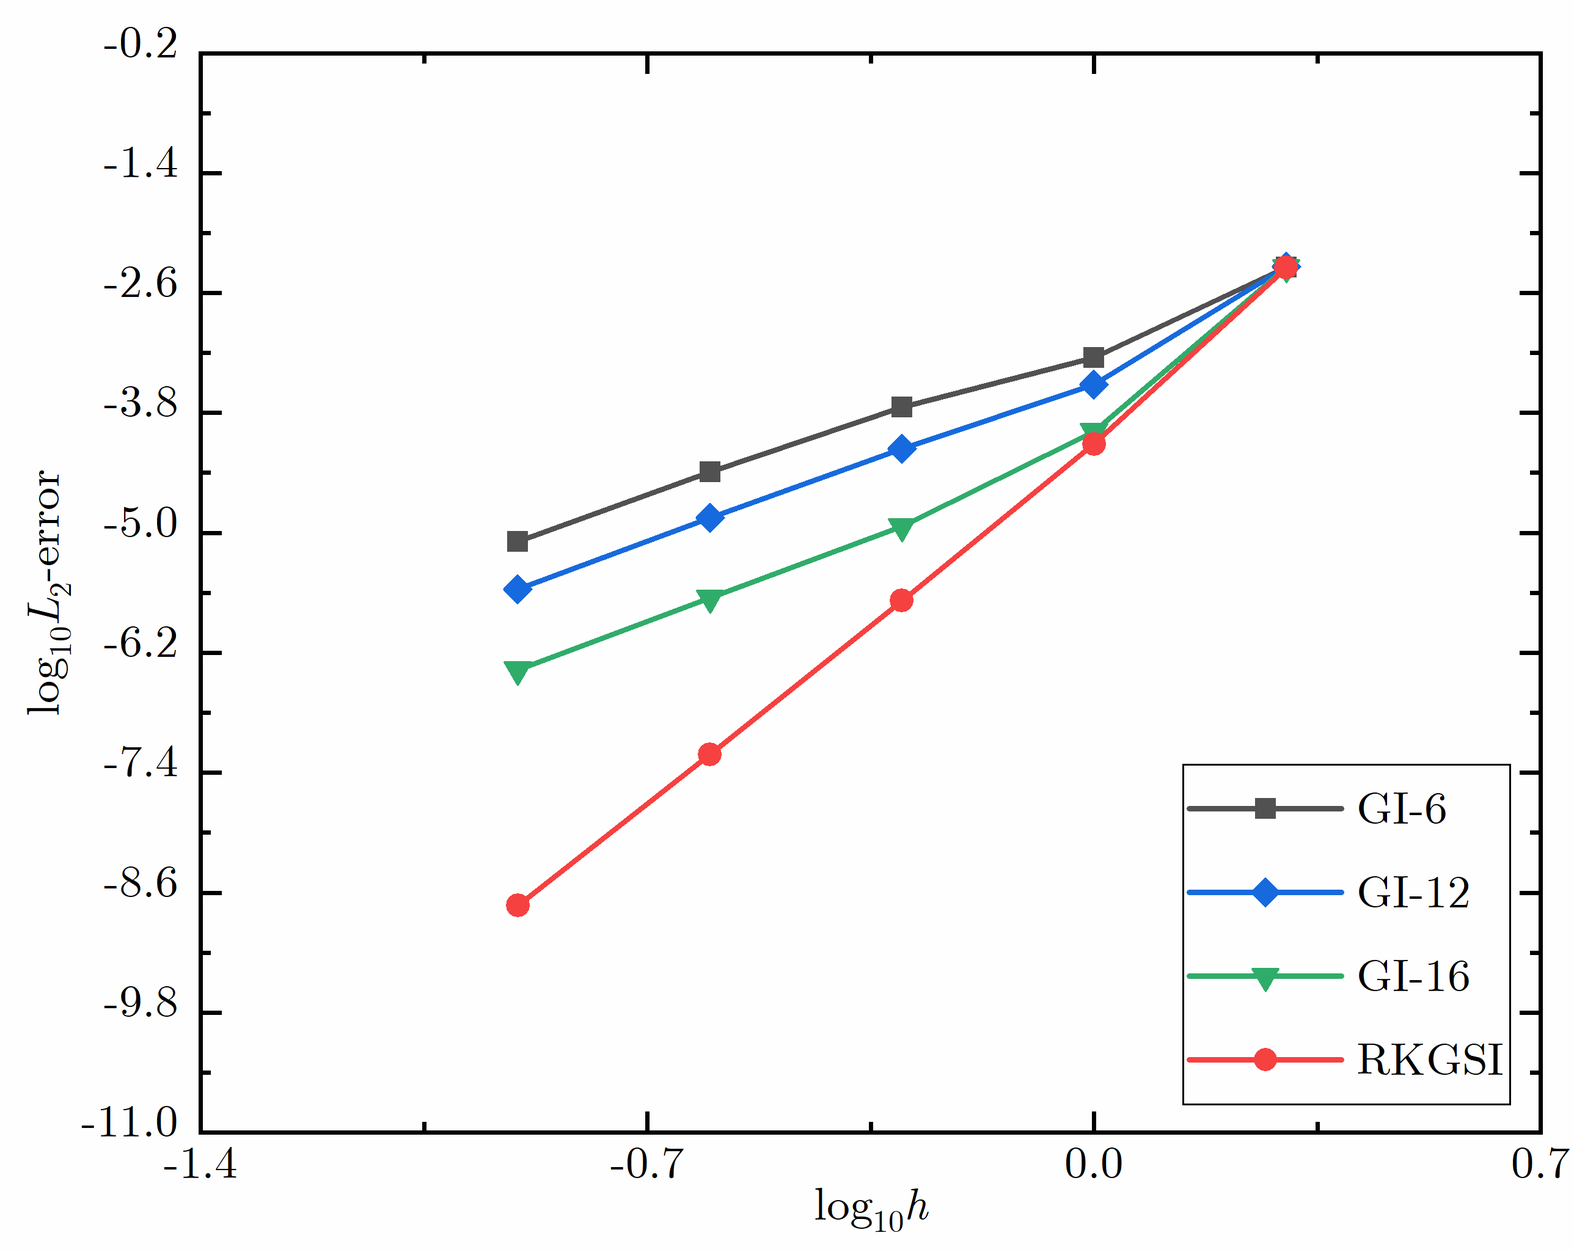
\includegraphics[width=0.55\textwidth]{figs/fig25.png}
\caption{$L_2$-error comparison for the 2D manufactured plate with $p=4$.}\label{fig:25}
\end{figure}

\begin{figure}[pos=htbp]
\centering
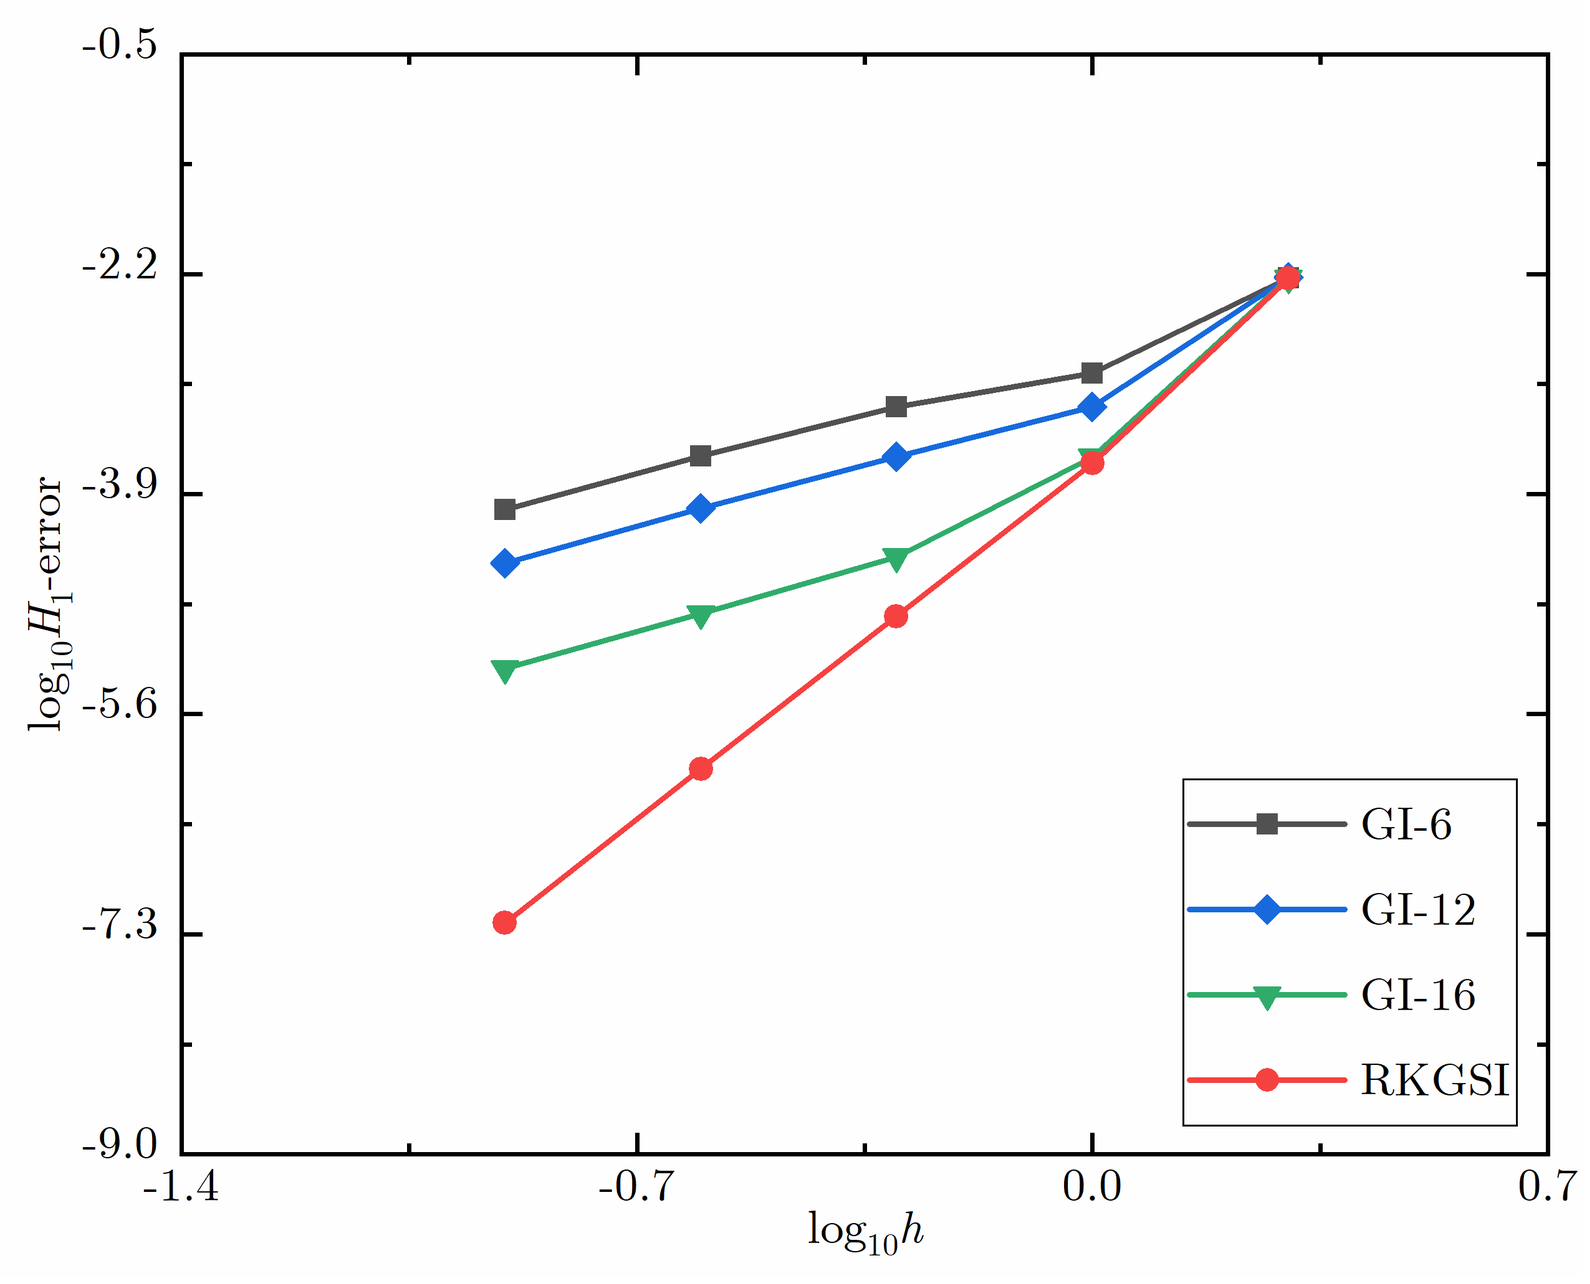
\includegraphics[width=0.55\textwidth]{figs/fig26.png}
\caption{$H_1$-error comparison for the 2D manufactured plate with $p=4$.}\label{fig:26}
\end{figure}

\begin{figure}[pos=htbp]
\centering
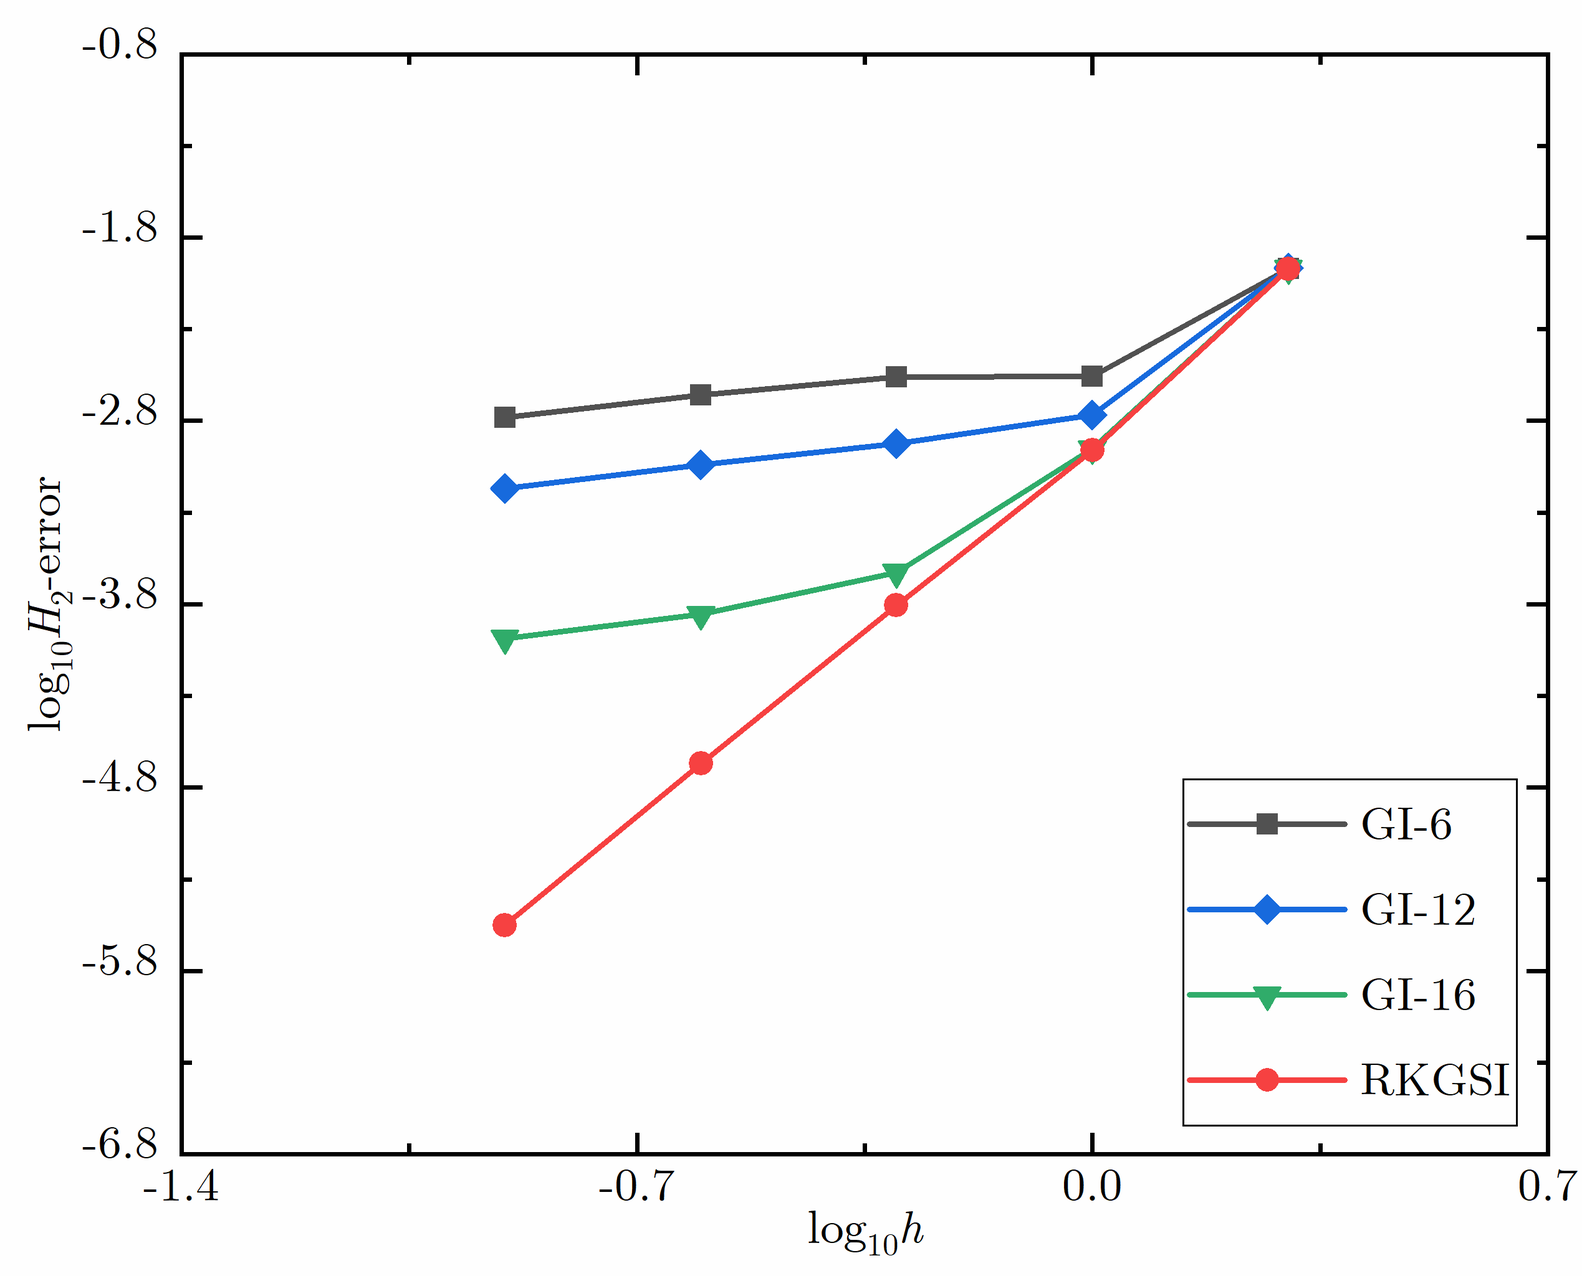
\includegraphics[width=0.55\textwidth]{figs/fig27.png}
\caption{$H_2$-error comparison for the 2D manufactured plate with $p=4$.}\label{fig:27}
\end{figure}
